\chapter[Comparaison d'explications locales]{Comparaison d'explications locales} \label{C3}

\boitemagique{Dans ce chapitre}{
    Nous traitons ici l'évaluation des explications. Trois protocoles sont proposés, afin d'évaluer le format et la méthode de génération des explications.
    L'application des différents protocoles met en avant leurs intérêts et limites.
    Les protocoles d'évaluation des méthodes de génération présentent une forte dépendance à la disponibilité d'une explication de référence de qualité.
}

% Quoi
Dans le chapitre précédent, nous avons conçu différentes illustrations d'explications, et appliqué plusieurs méthodes de générations d'explications pour un même format. Nous allons maintenant mettre en place des protocoles de comparaison de ces formats et méthodes, avec et sans utilisateurs.
L'application des protocoles montre leurs intérêts et limites respectives, notamment liées à la qualité des explications de référence.

% Plan
La collecte des retours utilisateurs est présenté en section~\ref{C3:test_u}. Nous recueillons les avis d'experts sur différentes illustrations, et nous développons des interfaces en conséquence. Enfin, nous présentons la collecte des préférences des experts du domaine.
Dans la section~\ref{C3:iou_expe} les méthodes sont comparées en se basant sur des métriques objectives, permettant de valider le respect de critères donnés. Cette expérimentation se fait sans utilisateurs.
Elle peut être menée rapidement et nécessite peu de prérequis.
Dans la section~\ref{C3:pus}, les utilisateurs cible sont intégrés à l'expérimentation, permettant de mesurer leurs préférences. Cette expérimentation nous permet de questionner la qualité des explications de références et la pertinence de la mesure utilisée en section~\ref{C3:iou_expe}.

\section{Collecte des retours des experts} \label{C3:test_u}
% quoi
Dans un premier temps nous présentons les collectes des retours des utilisateurs experts du cas d'usage LEGO.
% plan
En section~\ref{C3:discussion} nous présentons les analyses à chaud et discussions avec le panel d'experts autour des illustrations du chapitre 2.
Nous détaillons les interfaces créées grâce à ces retours en section~\ref{C3:solution} en précisant quelles solutions sont écartées, retenues, et quelles adaptations sont prises en compte.
En section~\ref{C2:collect_pref} nous présentons la collecte de préférences utilisateurs réalisée à partir de l'interface développée en section~\ref{C3:solution}.

\subsection{Test d'utilisabilité}\label{C3:discussion}

Le point avec les experts débute par plusieurs rappels permettant de s'assurer que les éléments de vocabulaire, objectifs et éléments fonctionnels sont bien partagés par tous. Nous rappelons quel est l'acte métier étudié, à l'aide d'un exemple qui nous servira tout au long de la présentation. Cela nous permet de dé-corréler l'analyse de l'interface de l'analyse métier. La discussion est basée sur les illustrations présentées en chapitre 2.

% Qui
% KAZBENNAOU Brahim - chargé relation entreprises - missionné DSI
% LECORBEILLER Eric - Manager de terrain
% PHAROSE Samuel & MAILHOL Sandrine - conseillers E
Les personnes identifiées pour ce test sont toutes expertes dans l'analyse de la qualité des offres d'emploi. Elles sont quatre, de métiers complémentaires. Ce panel est ainsi constitué d'un chargé de relations entreprises, un manager de terrain, et un conseiller et une conseillère à dominante entreprise.

Une fois les illustrations présentées, les experts donnent leurs avis sur chacune des propositions, discutent entre eux et mettent en avant les éléments qui leur manquent.
L'objectif de cette phase de discussion est de faire le tri sur les propositions et leurs variantes, ajuster les maquettes au besoin des personnes interrogées, et palier aux éventuels oublis et manques.
Nous passons en revue chaque proposition et les nouvelles idées sont traitées à part.

\paragraph{Explication par phrase} La mise en avant de phrases a été très appréciée par le panel d'utilisateurs. Iels apprécient le contexte global que fournit la phrase entière, notamment lorsque le descriptif de l'offre est long.
Parmi les variantes, le surlignage est bien perçu tandis que le soulignage n'est pas apprécié. La bulle d'informations au survol de la phrase est fortement rejetée.

\paragraph{Explication par mot} La mise en avant de mots a été bien reçue par les utilisateurs. Le système précédent fournissant des mots ou expressions également, cette solution ressemble fortement à ce qu'iels connaissent déjà, réduisant ainsi le cout de changement. Comme pour les phrases, la variante de surlignage des mots est plébiscitée, et les bulles lors du survol sont fortement rejetées. Les utilisateurs préfèrent le surlignage dans le texte plutôt que le bandeau à part. Si ce bandeau correspond à l'interface actuelle de DUNE (cf. figure~\ref{fig:ihm_DUNE}), le surlignage direct réduit les allers-retours visuels.

\paragraph{Exemple} L'explication par l'exemple n'a pas convaincu les utilisateurs. Iels ne voient pas l'intérêt de montrer une phrase proche et toujours rejetée, car cette phrase ne donne pas d'information intéressante. Les éléments communs pourraient être détectés par le surlignage de mots et le contexte global pourrait être mis en avant en surlignant la phrase rejetée. L'exemple ajoute de la lecture sans avantage comparé aux deux maquettes énoncées. Il n'apporte rien par rapport à leur expertise.

\paragraph{Contre-exemple} Les explications par le contre-exemple en revanche ont été accueillies avec enthousiasme. Les experts ont trouvé un réel intérêt fonctionnel à cette maquette, car le contre-exemple peut être considéré comme une proposition de correction, si la phrase proposée est assez proche sémantiquement de la phrase en rejet. Du point de vue de l'acte métier, ce serait un gain de temps d'avoir seulement à valider ou ajuster la proposition de correction.

\paragraph{Proposition} De nouvelles idées ont émergé en se basant sur les explications par l'exemple. Les experts proposent de fournir des explications sous forme de règles générales, en se référant au Guide d'Aide à la Rédaction des Offres (GARO). Ce document référence de 128 pages résume les bonnes pratiques et redirige si besoin vers des documentations plus complètes. Le GARO est long, et un récapitulatif affiché à chaque rejet pourrait éviter dans de nombreux cas de devoir s'y référer.
Ce type d'explication serait particulièrement bienvenu dans le cadre de l'accompagnement d'employés novices sur la rédaction des offres.

Ces retours à chaud récupérés et consignés permettent la prise de décision sur les propositions, afin de les ajuster, abandonner, ou créer. Les personnes interrogées ont ainsi exprimé leur préférence pour les explications au niveau de la phrase, puis des mots et contre-exemples, puis des règles.

\subsection{Solutions écartées et retenues}\label{C3:solution}

Dans les différentes variantes proposées, deux points font l'unanimité des personnes interrogées. Premièrement les bulles d'aides apparaissant en survolant des éléments ne sont pas appréciées. Deuxièmement, le surlignage des éléments mis en avant est apprécié, et détrône l'interface d'origine avec son bandeau d'informations.

\paragraph{Simplification du problème}
Cette discussion a acté la simplification principale des travaux menés : se limiter à la classification mono-label, multi-classe. C'est à dire, pour une phrase, ne considérer qu'un seul motif de rejet.
Du point de vue fonctionnel, un utilisateur expert traitera probablement toutes les irrégularités d'un coup, où les éliminera une à une au fil de la mise à jour des motifs de rejet de la part du système.
Cette simplification technique n'a donc pas d'impact négatif fonctionnel.
De même, les personnes interrogées ont soulevé une inquiétude quant à la superposition des informations mises en avant, notamment par le soulignage, dans les rares cas concernés.

\paragraph{Règles générales}
Les utilisateurs proposent de remplacer les explications par l'exemple par des règles plus générales, apportant des précisions sur les bonnes pratiques consignées dans le GARO. En effet, ce type d'information est particulièrement adapté pour les personnes en formation, ou pour les cas rares ou ambigus. En donnant de précisions ou en redirigeant vers les bonnes pages du GARO, les rappels de règles permettent de gagner du temps et capitaliser sur des références déjà existantes.

La difficulté technique de l'implémentation d'un système d'explication n'est pas corrélée à son utilité perçue par les utilisateurs.
Ainsi la préférence des personnes interrogées, basée sur les maquettes, est dans l'ordre de préférence décroissante : surlignage par phrase, puis à égalité mot surlignés et contre-exemples, et enfin l'affichage des règles.
La difficulté quant à elle, a été, dans l'ordre décroissant : Génération de contre-exemples, surlignage des mots, affichage de règles et surlignage de phrases.

% demandes générales :
De manière globale, les retours des experts font écho à leur préoccupation principale : aller vite. Soit en ajoutant de l'information ou des précisions manquantes pour éviter d'aller chercher ces informations ailleurs, soit en faisant gagner du temps en proposant directement une correction. D'un point de vue utilisateur, surligner les mots est plus agréable que les phrases lorsque ces dernières sont longues.

\begin{figure}[htpb!]
    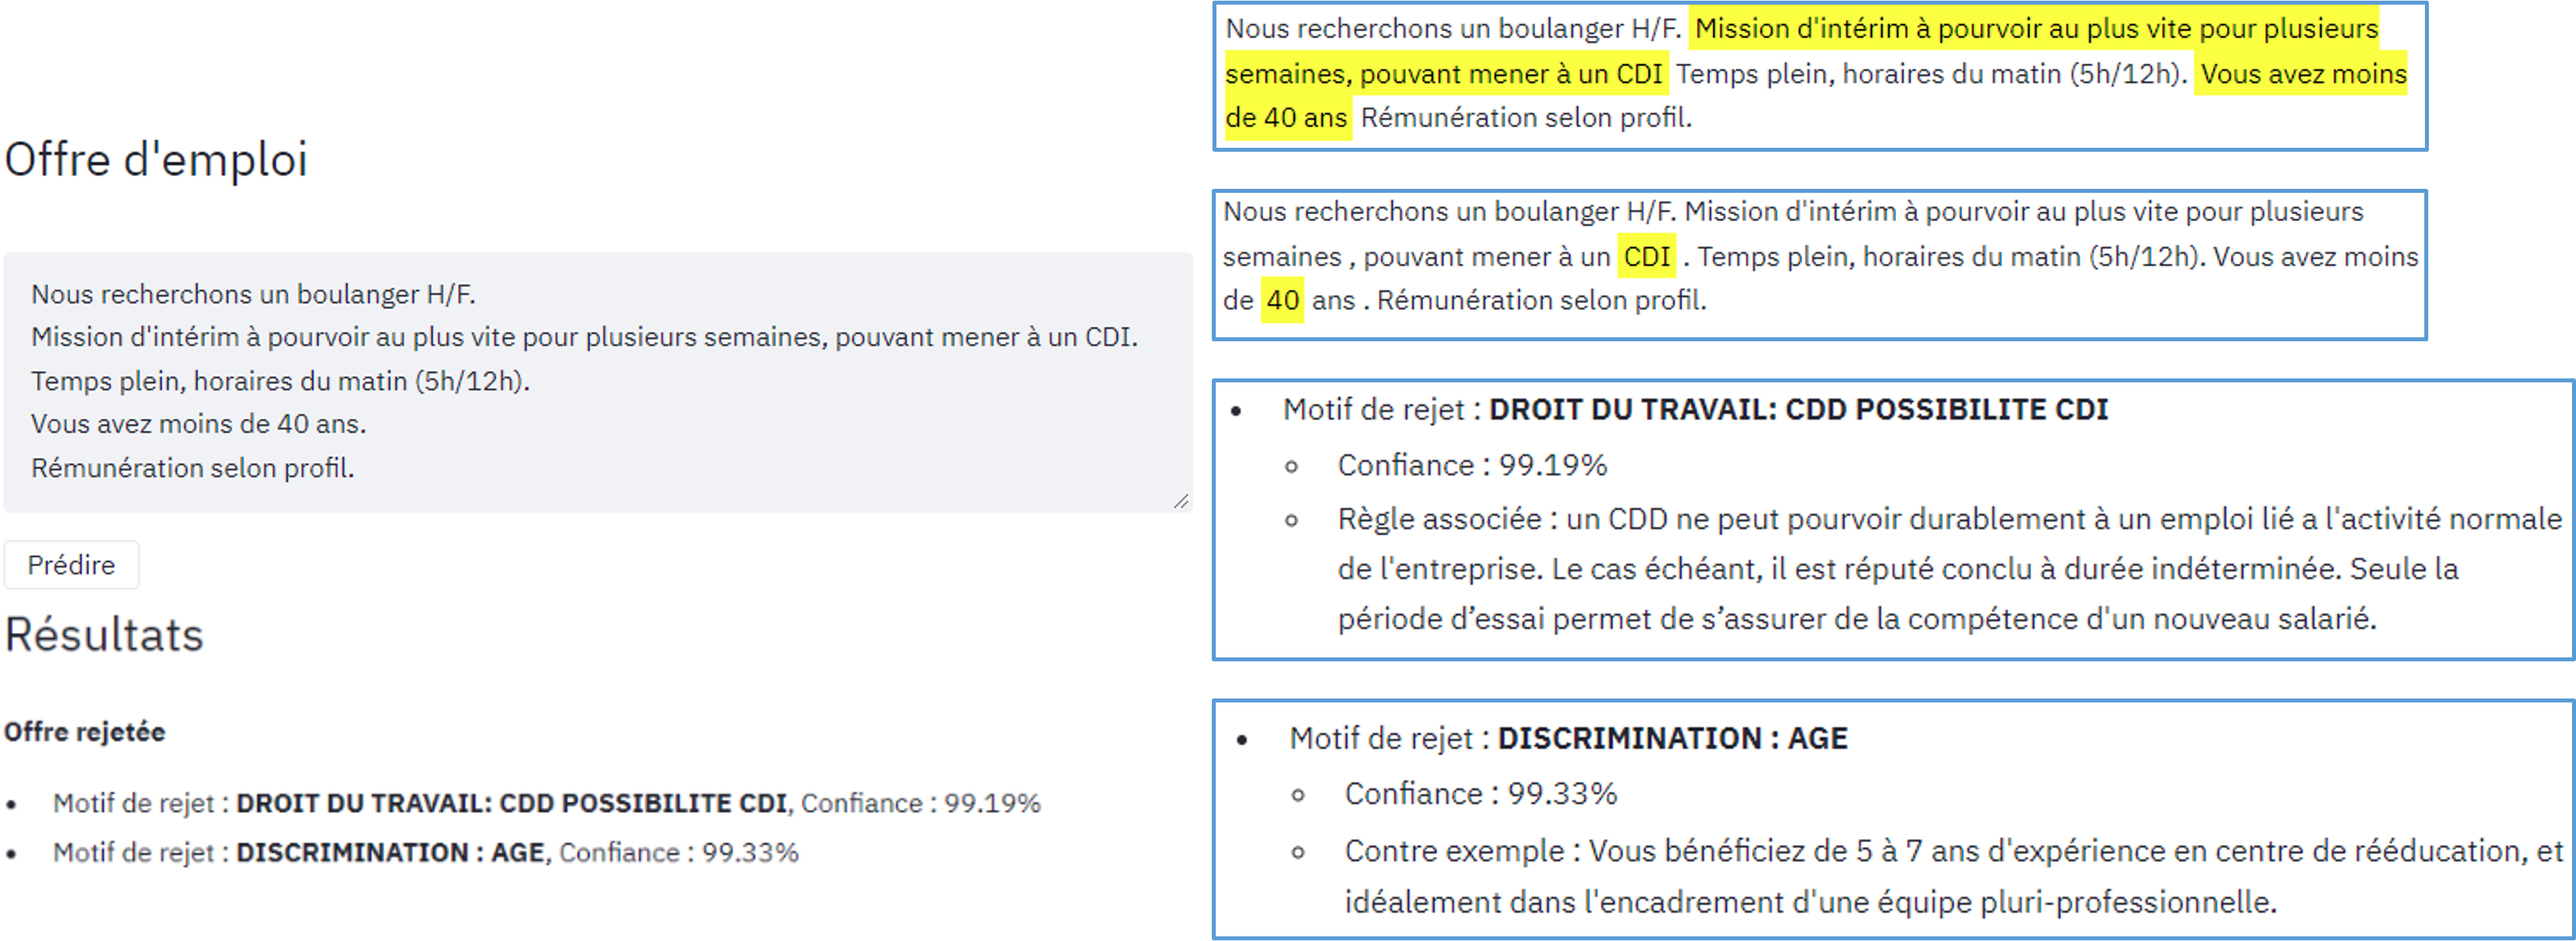
\includegraphics[width=\textwidth]{./S2-Explicabilite_locale/figures/explications_locales.png}
    \caption{Montage présentant un condensé des différentes interfaces développées.}
    \label{fig:explications_locales}
\end{figure}

\paragraph{Explication par phrase} Cette explication consiste à surligner l'ensemble des phrases rejetées par le système, comme illustré dans la figure~\ref{fig:demo_phrase}.
% comment
\begin{itemize}
    \item Si le modèle d'IA renvoie un motif de rejet pour une phrase, alors le texte est réaffiché dans l'encart ``Résultats'', et la phrase en question est surlignée.
    \item Si plusieurs phrases sont surlignées, le texte n'apparaît qu'une fois et contient toutes les phrases surlignées.
    \item Les motifs de rejets sont affichés dans l'ordre d'apparition dans l'offre.
\end{itemize}
Ainsi, dans la figure~\ref{fig:demo_phrase}, la phrase ``Mission d'intérim à pourvoir [...] pouvant mener à un CDI.'' est associée au premier motif de rejet \textit{Droit du travail : CDD possibilité CDI}.

\begin{figure}[htpb!]
 \centering
 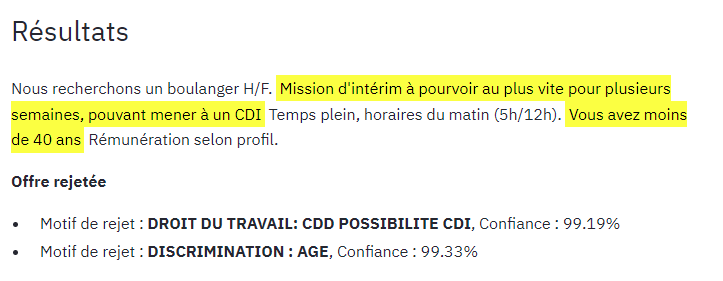
\includegraphics[width=0.7\textwidth]{S2-Explicabilite_locale/figures/demo_phrase.png}
 \caption{Démonstrateur présentant l'interface pour l'explication par phrase(s) surlignée(s).}
 \label{fig:demo_phrase}
\end{figure}

% Avantage
Ce type d'explication a l'avantage d'être peu couteux à mettre en place. Il est rapide, car ne nécessite pas de calcul supplémentaire après inférence. Il met en avant le contexte du rejet, laissant le soin à l'utilisateur d'analyser la ou les phrases en rejet.
% inconvénient
Toutefois, en surlignant toute la phase, la visualisation est peu précise. C'est un problème si une phrase est longue, ou si un texte est mal formaté et ne comporte pas de ponctuation permettant de séparer les phrases. De même, le comportement interne du modèle n'est pas explicité.

\paragraph{Explication mot à mot} Sur le même principe que l'explication par phrase, l'explication par mot surligne le ou les mots menant à la décision de rejet par le système. Comme illustré dans les figures~\ref{fig:demo_mot}, pour chaque phrase rejetée par le système, les mots sont surlignés dans le texte. Les motifs de rejets sont toujours affichés dans l'ordre d'apparition. Les mots à surligner sont déterminés par une méthode d'explication basée sur les importances de variables, ici avec la méthode d'attention. Plus de détails sur la sélection de ces mots sont donnés en section~\ref{C2:explications}. Sur la figure~\ref{fig:demo_mot_1}, le motif de rejet \textit{Droit du travail : CDD possibilité CDI} est ainsi lié à la présence du mot ``CDI'' dans le texte. À noter que la seule présence du mot n'est pas une explication suffisante, le contexte étant également pris en compte. Par exemple dans la figure~\ref{fig:demo_mot_2}, la seconde phrase n'est plus rejetée mais comporte toujours le mot ``CDI''.

\begin{figure}[htpb!]
    \centering
    \begin{subfigure}[b]{0.48\textwidth}
        \centering 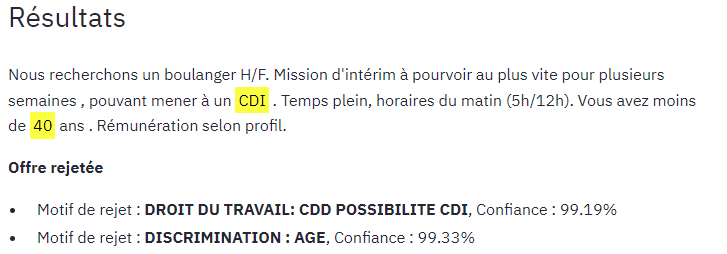
\includegraphics[width=\textwidth]{S2-Explicabilite_locale/figures/demo_mot.png}
        \caption{Explication pour deux phrases en rejet}
        \label{fig:demo_mot_1}
    \end{subfigure}
    ~
    \begin{subfigure}[b]{0.48\textwidth}
        \centering 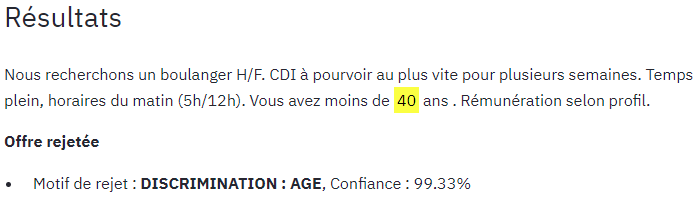
\includegraphics[width=\textwidth]{S2-Explicabilite_locale/figures/demo_mot_2.png}
        \caption{Explication pour une seule phrase rejetée}
        \label{fig:demo_mot_2}
    \end{subfigure}
    ~
    \caption{Démonstrateur présentant l'explication mot à mot
 }\label{fig:demo_mot}
\end{figure}

% Avantage
L'explication mot à mot est précise, et reflète le comportement du modèle d'IA étudié, plus ou moins fidèlement selon la méthode d'explication employée.
% inconvénient
Néanmoins, ce type d'explication nécessite un calcul supplémentaire, afin de déterminer les mots responsables du rejet. Il complexifie l'outil, et ajoute un délai pour afficher l'explication.

\paragraph{Règle} Afficher une règle métier constitue une explication courte, extraite des documents de référence et associée au motif de rejet détecté. Cette interface réalisée à la demande des utilisateurs est présentée en figure~\ref{fig:demo_regle}.
% comment
Lors de la détection d'une phrase rejetée, le motif de rejet est affiché dans l'encart de résultats. Une règle associée est affichée juste en dessous. La figure~\ref{fig:demo_regle} montre l'affichage de deux motifs de rejets et les règles associées. Une règle est toujours la même pour un motif donné. Elle est définie manuellement pour chacun des 27 motifs de rejet, en résumant brièvement les informations présentes dans le GARO.

\begin{figure}[htpb!]
 \centering
 
\includegraphics[width=0.7\textwidth]{S2-Explicabilite_locale/figures/demo_regle.png}
 \caption{Démonstrateur pour l'interface d'explication par la règle métier.}
 \label{fig:demo_regle}
\end{figure}

% Avantage
Cette interface a l'avantage d'être facile à mettre en place d'un point de vue technique. Son affichage est rapide, car elle ne nécessite pas de calcul. Elle est plus généralisable qu'un exemple. Elle est basée sur l'expertise métier et les documents de référence, ce qui la rend particulièrement adapté aux utilisateurs non experts, en leur fournissant un premier niveau d'information.
% inconvénient
En contrepartie, cette interface fournit des explications peu précises, parfois insuffisantes dans le cadre de cas délicats. Dans sa version implémentée, elle nécessite un travail manuel afin de résumer le document de référence.

\paragraph{Contre-exemple} On peut également associer une phrase rejetée à une phrase proche de celle-ci, mais acceptée par le système. La figure~\ref{fig:demo_cfe} présente cette interface.
% comment
La création des contre-exemples est une preuve de concept. C'est une version développée dans un temps court, peu efficiente, mais qui donne des pistes de réflexion. Les contre-exemples sont récupérés dans une base restreinte de $100$ phrases légales, appelés ci-après \textit{candidats}. La phrase illégale ainsi que tous les candidats sont rapprochés en les vectorisant via un plongement de mots, puis en rapprochant ces vecteurs avec une distance sémantique : la distance cosinus entre les vecteurs représentant les phrases. Le contre-exemple est la phrase légale ayant la distance cosinus minimale avec la phrase rejetée.  % TODO vérifier

\begin{figure}[htpb!]
\centering

\includegraphics[width=0.7\textwidth]{S2-Explicabilite_locale/figures/demo_cfe.png}
\caption{Démonstrateur pour l'interface d'explication par le contre-exemple.}
\label{fig:demo_cfe}
\end{figure}

% Avantage
Ce type d'explication a l'avantage d'être contrastif, une explication bien perçue par les humains.  %cite.. Miller ?
Le contre-exemple est extrait d'un ensemble de phrases réelles, ce qui réduit le risque d'explications hors distributions, ressemblant à un élément réaliste, mais trompant le modèle d'intelligence artificielle.
Enfin, dans ce cas d'usage, fournir un contre-exemple revient à proposer une correction automatique de l'offre, pour peu que la phrase de contre-exemple soit assez proche de celle d'origine.
% inconvénient
L'inconvénient de cette approche est qu'elle nécessite de bons candidats au contre-exemple. Il est nécessaire de trouver un moyen de filtrer ces bons candidats, car la comparaison par paires de phrase est couteuse en calculs. De même, l'explication avec des candidats qui sont peu intéressants car trop spécifique, ou trop éloignés du sens sémantique d'origine, sont peu intéressants pour les utilisateurs et pourraient générer plus de frustration qu'en enlever.

\subsection{Préférences des utilisateurs} \label{C2:collect_pref}

% Quoi
Nous utilisons l'interface d'explications par surlignage des mots précédemment présentée afin de recueillir les préférences des experts et expertes du domaine. Plusieurs méthodes de collecte sont possibles :
\begin{itemize}
    \item La notation les explications, par exemple sur 5 points. Cela permet de donner une valeur absolue aux méthodes évaluées, mais implique la création d'un barème mental propre à chaque utilisateur.
    \item Le tri des explications. L'utilisateur a ainsi une vision d'ensemble des explications. Cette méthode permet d'ordonner des explications courtes.
    \item La comparaison par paire d'explications. Cette méthode est préférable pour ordonner des explications longues.
\end{itemize}

Nous nous intéressons ici uniquement à l'ordre de préférence et n'avons donc pas besoin de cette valeur absolue. Nous présentons des phrases pouvant être longues, nous privilégions la comparaison par paires d'explication.
C'est un outil efficace car il est plus facile pour un humain de dire quelle explication iel préfère, plutôt que donner une note.

\paragraph{Interface présentée}
Pour recueillir leurs préférences, les utilisateurs se voient présenter deux fois la même phrase dans l'interface d'explication par surlignage des mots importants. La classification du modèle d'IA et une explication par la règle sont également présentées. Ces éléments sont visibles sur la Figure~\ref{fig:expe_ui} dans les deux zones sur fond blanc.

Les utilisateurs sont invités à choisir l'explication répondant à la question : ``Quelle est l'explication la plus utile pour comprendre l'alerte ?'', l'alerte étant la raison du rejet donné par le modèle. Comme le montre la Figure~\ref{fig:expe_ui}, la question est affichée en haut de l'écran pendant toute l'expérience.
La réponse peut être une erreur du modèle. Dans ce cas, les explications fournies peuvent sembler hors sujet aux utilisateurs, comme discuté dans la section~\ref{C2:ground_truth}.
L'explication peut être vide, ce qui signifie qu'il n'y a pas de mot mis en évidence. Si les utilisateurs ne perçoivent aucune préférence entre deux explications, on leur demande d'en choisir une selon leur sentiment subjectif. Comme plusieurs utilisateurs évaluent les mêmes phrases, ces cas apparaîtront dans les données comme des choix difficiles, où aucune explication ne ressort.

\begin{figure}[h!tpb]
  \setlength{\belowcaptionskip}{-20pt}
  \begin{center}
    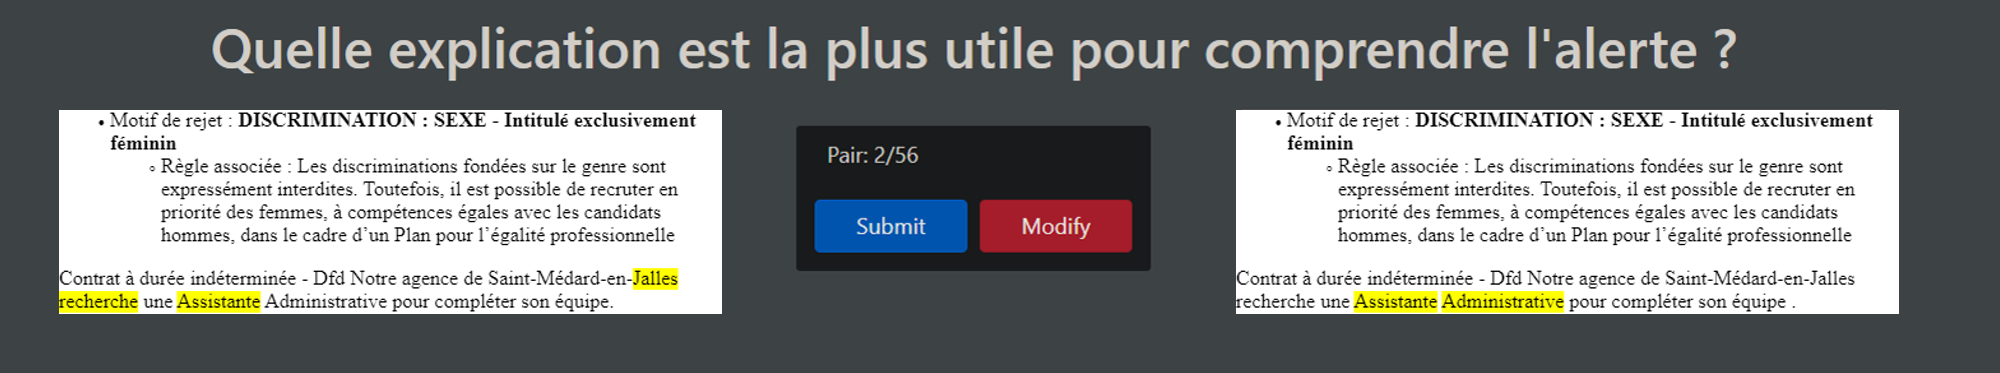
\includegraphics[width=\textwidth]{S3-Comparaison_de_methodes/figures/user_experiment_interface.png}
    \caption{L'interface de l'expérience. Les utilisateurs doivent choisir entre deux explications présentées celle qu'iels préfèrent. La raison du rejet et la règle associée sont affichées. Les explications sont des mots surlignés.}\label{fig:expe_ui}
  \end{center}
\end{figure}

% le profil des utilisateurs
\paragraph{Contraintes expérimentales}
Pour lutter contre le biais d'apprentissage, 14 utilisateurs ont été recrutés par le biais du réseau interne de \textit{P\^ole Emploi}. Ce sont des employés spécialisés dans l’accompagnement des recruteurs, iels possèdent donc une expertise du domaine. Iels sont particulièrement habitués à rédiger et à éditer des offres d'emploi et travaillent depuis de nombreuses années avec une ancienne version de notre solution d'IA basée sur des expressions régulières (regex) qui lèvent des alertes légales. Par conséquent, les utilisateurs de cette expérience sont déjà conscients des cas possibles menant à des faux positifs et négatifs pour le rejet automatique d'offres d'emploi. En définitive, ces experts ne sont pas sujets à des erreurs dues à la découverte du cas d'usage.

% Les précautions
Nous avons également pris en compte la concentration, la fatigue et la faible disponibilité des utilisateurs. Les précautions suivantes ont été prises.
\begin{itemize}
    \item La collecte est divisée en 9 sessions courtes, de 30 minutes chacune.
    \item Les sources de notification telles que les téléphones portables ou les logiciels de communicationsont mises en sourdine.
    \item Chaque utilisateur voit les paires dans un ordre différent.
    \item La tâche donnée est simple, l'interface possède très peu d'éléments, comme le montre la Figure~\ref{fig:expe_ui}.
    \item La tâche de comparaison est conçue pour être réalisée de manière autonome.
    \item L'expérience ne nécessite pas de conditions spécifiques telles que le niveau de lumière ou la colorimétrie de l'écran.
    \item En cas de blocage, les utilisateurs peuvent poser des questions par téléphone ou via leur outil habituel de messagerie instantanée.
\end{itemize}

% Résultat
Cette expérimentation a permis de recueillir les préférences de 14 utilisateurs sur 109 phrases. Tous n'ont pas eu la possibilité d'effectuer la totalité des 9 sessions.
104 sessions ont été réalisé sur les 126, soit $83\%$ des comparaisons à effectuer.
9 participants ont réalisé la totalité des sessions. Eut égard de la difficulté de mobiliser les experts et expertes, il était prévu que toutes les comparaisons ne soient pas effectuées.

% conclusion section
% rappel objectif
Nous avons présenté le test d'utilisabilité, de son déroulement en section~\ref{C3:discussion} aux conclusions tirées des entretiens en section~\ref{C3:solution}. Les retours des utilisateurs nous ont aidés à définir des interfaces mieux adaptées à leur besoins. La figure~\ref{fig:explications_locales} montre les interfaces finales conçues dans le démonstrateur présenté dans le chapitre précédent.
La section suivante présente l'évaluation de méthodes d'explications sans utilisateurs.

\section{\'Evaluation sans utilisateurs} \label{C3:iou_expe}

% Quoi
L'évaluation présentée fournit de premiers résultats, lorsqu'il n'y a pas d'utilisateur expert du domaine disponible. Nous cherchons à savoir quelle méthode d'explication convient le mieux à chaque cas d'usage dans son contexte donné.
Ces expérimentations sans utilisateurs permettent de valider des propriétés telles que la concision ou la représentativité, ainsi que décrites en introduction.

% Comment
Nous divisons notre problème en deux questions.
\begin{enumerate}
    \item Cette explication est-elle proche d'une explication idéale ? Nous répondons à cette question de façon quantitative, en mesurant la proximité entre explications générées et de référence.
    \item Lorsqu'il n'y a pas de référence, comment évaluer les méthodes d'explication ? Nous optons pour une approche qualitative, en filtrant pour analyser uniquement les cas où les explications générées sont peu similaires.
\end{enumerate}
Les réponses à ces deux questions permettent d'établir une première évaluation des méthodes appliquées.
Nous appliquons ce protocole aux explications générées dans le chapitre précédent.
Nous nous assurerons notamment que les explications sont concises, fidèles et adaptées aux receveurs
% plan
Nous présentons dans la section~\ref{C3:qt_metric} l'étude quantitative des explications, puis en section~\ref{C3:ql} l'analyse qualitative.

\subsection{Spécificités du cas d'usage Yelp} \label{C3:cu_yelp}

Le cas d'usage Yelp est utilisé afin de généraliser notre protocole. Il est basé sur l'application du même nom permettant à des utilisateurs de noter et donner des avis sur des commerces dont iels ont été clients. La tâche est de retrouver le nombre d'étoiles, entre 1 et 5, associées à un avis utilisateur. Si ce n'est la langue qui est l'anglais, Yelp est, comme le cas d'usage LEGO, un problème de classification de texte, multi-label, multi-classe. L'ensemble d'entraînement contient $453 600$ avis.

% Comment
Ce cas d'usage requiert une version spécifique du réseau d'attention. Les textes sont vectorisés avec un plongement de mots spécifique à l'anglais, générant des vecteurs de 100 dimensions, et basé sur Wikipédia dans sa version anglophone\footnote{\url{https://wikipedia2vec.github.io/wikipedia2vec/pretrained/}}. L'optimiseur est Adam, avec un taux d'apprentissage de $0,0005$.
Ce réseau obtient une précision de $74,63\%$ sur son ensemble de test. En comparaison, les auteurs de~\cite{Lin2017} présentent dans leur article une précision de $64.21\%$ sur leur propre jeu de test.

% comparaison des modèles pour générer les explications avec YELP et LEGO
L'architecture précise du modèle à attention est présentée en C2, pour le cas d'usage LEGO. Ici, nous présentons les différences entre les deux architectures.
\begin{table}
\caption{Comparaison des architectures des réseaux de neurones pour YELP par rapport à LEGO.}\label{model_architecture}
\begin{tabular}{|l|p{0.23\textwidth}|p{0.1\textwidth}|p{0.1\textwidth}|p{0.42\textwidth}|}
\hline
\textbf{ID} & \textbf{Type de couche} & \textbf{YELP} & \textbf{LEGO} & \textbf{Commentaires} \\ \hline
1 & Couche d'entrée    & 300  & 80  & La taille est le nombre de mots dans les textes \\ \hline
2 & Plongement de mots & 100  & 300 & Plongement de mots Word2vec\\ \hline
3 & Bi-LSTM            & $u=$150  & $u=$50  & La sortie est la matrice d'états cachés H \\ \hline
4 & Couche dense 0     & $d_a=$350  & $d_a=$300 & Activation $tanh$ \\ \hline
5 & Couche dense 1     & $r=$1    & $r=$1   &  La sortie est la matrice d'attention A \\ \hline
6 & Représentation     & sortie: $[2u,r]$ & sortie: $[2u,r]$   & Combinaison de l'attention et de la couche cachée, $M=A^T*H$  \\ \hline
7 & Couche dense 2     & 1000 &  $\emptyset$   & Activation $ReLu$ , pour Yelp uniquement \\ \hline
8 & Couche dense 3     & 5    & 28  & Couche de sortie \\ \hline
\end{tabular}
\end{table}

Deux explications sont extraites de ce modèle : les explications par les ancres et les explications d'attention avec un seuil $t=0,15$. Le tableau~\ref{exemple_yelp} illustre ces explications sur une évaluation du jeu de données Yelp. L'étude utilisateur n'est pas réalisée dans ce cas d'usage, il n'y a donc qu'un seul seuil d'attention généré. Comme l'explication des ancres sur de grands textes entraîne souvent des problèmes de mémoire, les ancres ont été appliquées à un sous-ensemble de 1060 évaluations les plus courtes sur les 2653 évaluations de l'ensemble de test complet.

\begin{table}[h!tpb]
\caption{Exemples extraits de Yelp : deux critiques avec des notes et des explications pour les ancres et les méthodes d'attention. Le texte est au-dessus des autres informations.}\label{exemple_yelp}
\begin{tabular}{|p{0.19\textwidth}|p{0.18\textwidth}|l|}
\cline{1-3}
\textbf{Note} & \textbf{Ancres} & \textbf{Attention 0.15} \\ \hline
\multicolumn{3}{|p{0.95\textwidth}|}{``Wow! Superb Maids did an amazing job cleaning my house. They stayed as long as it took to make sure everything was immaculate. I will be using them on a regular basis.''}\\ \hline
5 & {[}{]} &  ['superb', 'amazing', 'everything'] \\ \cline{1-3}
\multicolumn{3}{|p{0.95\textwidth}|}{``For the record, this place is not gay friendly. Very homophobic and sad for 2019. Avoid at all costs''} \\ \hline
1 & ['not'] & ['record', 'not', 'homophobic', 'sad', 'avoid'] \\ \cline{1-3}
\end{tabular}
\end{table}

Une fois les explications générées pour les deux cas d'usage, il reste un dernier type d'explication à récupérer pour mener à bien la suite des expérimentations : les explications des utilisateurs.

\subsection{Analyse quantitative} \label{C3:qt_metric}

% quoi
Dans un premier temps nous cherchons à répondre à la première question : ``Cette explication est-elle proche d'une explication idéale ?''.
Pour cela, nous comparons les explications générées à l'explication de référence,  considérée comme le meilleur résultat possible.
%pourquoi
Ces mesures ont pour objectif de savoir quelles sont les explications les plus fidèles, adaptées au receveur et concises.

%comment
La concision des explications est mesurée par le nombre de mots des explications.
Pour quantifier l'adaptation au receveur et la fidélité, les explications générées sont comparées à la référence (voir section~\ref{C2:ground_truth}). Une métrique simple de similarité entre deux ensembles a été reprise, l'IOU, et est utilisée parmi d'autres métriques connues (précision, score F1...).
Tel qu'utilisé dans~\cite{Bau2017}, l'IOU, l'exactitude et le score F1 sont également comparés, ainsi que le rappel et la précision utilisés dans le score F1. Le rappel est une mesure intéressante car elle n'est pas affectée par les vrais négatifs

% résultats
La concision est peu différenciante pour Yelp, les longueurs moyennes des explications étant similaires, 2,34 et 2,13 mots pour les ancres et l'attention respectivement.
Pour LEGO, les explications basées sur les ancres sont en moyenne plus courtes que celles basées sur l'attention. Les longueurs moyennes sont respectivement de 0,15 et 0,33 mots dans l'ensemble de test. La valeur moyenne est faible en raison des explications vides.
Ces mesures comparent la référence aux explications générées pour le jeu de données LEGO - Bonnes Prédictions (BP). Pour obtenir des mesures équitables, les mots vides ne sont pas pris en compte. L'évaluation du modèle n'étant pas le but de cette expérimentation, le jeu de test utilisé est le jeu de données LEGO - BP de 147 phrases correctement prédites.

\begin{table}[h!tpb]
  \centering
%  \addtolength{\parskip}{-0.5mm}
\caption{Comparaison des explications générées avec la référence, jeu de données LEGO BP. Les meilleurs résultats sont en gras. L'attention obtient des résultats légèrement meilleurs.}\label{anchors_gt_lego_success}
\begin{tabular}{|l|l|c|c|}
  \hline
  \textbf{Mesure} & \textbf{Ancres} & \textbf{Attention} \\ \hline
  % IOU           & 0.938 & 0.930 \\ \hline
  % Acc           & 0.980 & 0.973 \\ \hline
  % Recall        & 0.970 & 0.976 \\ \hline
  % Précision     & 0.961 & 0.943 \\ \hline
  % F1            & 0.965 & 0.959 \\ \hline
  IOU             & $0,94$ & $0,93$ \\ \hline
  Taux de reconnaissance & $0,98$ & $0,97$ \\ \hline
  Rappel          & $0,97$ & $0,98$ \\ \hline
  Précision       & $0,96$ & $0,94$ \\ \hline
  F1              & $0,97$ & $0,96$ \\ \hline
\end{tabular}
\end{table}

Les résultats de toutes les métriques pour le cas d'usage LEGO sont affichés dans le tableau~\ref{anchors_gt_lego_success}. Dans l'ensemble, comparées à la référence, les deux méthodes de génération d'explication obtiennent des résultats similaires, cf. Tableau~\ref{anchors_gt_lego_success}.
Les scores sont élevés, en partie à cause du nombre de phrases non rejetées dans le jeu de données LEGO - BP : 131. Ces instances n'ont pas d'explication, les différentes métriques sont dans ce cas égales à 1.

% analyse
Les ancres et l'attention sont également comparées les unes aux autres. En l'absence de référence, les métriques telles que la précision et le score F1 ne sont pas pertinentes. Une IOU élevée indique que les explications sont similaires dans les deux méthodes. L'IOU entre les ancres et l'attention est de $0,92$, ce qui indique qu'elles donnent des résultats similaires. Pour le cas d'usage LEGO, les explications des ancres et de l'attention sont toutes deux similaires et proches de l'explication idéale.

% Petit point sur YELP
Comme il n'y a pas de documentation ni d'expert du domaine pour le cas d'usage Yelp, il n'y a pas de référence pour son jeu de données. Par conséquent, la comparaison n'est possible qu'entre les ancres et les explications d'attention. L'IOU indique si les explications générées sont similaires. La moyenne de l’IOU sur l'ensemble de test réussi est de $0,23$, ce qui montre de fortes différences entre les deux méthodes d'explication. Cela peut s'expliquer par les longs textes et le vaste vocabulaire attendu dans les explications. Par conséquent, pour évaluer les méthodes d'explication dans le cas d'usage de Yelp, une analyse qualitative est nécessaire.

En définitive, l'analyse quantitative donne une première analyse sur chaque cas d'usage. Pour LEGO, les ancres sont plus concises, et aussi fidèles et adaptées que l'attention. Pour Yelp, les deux méthodes sont proches en concision, mais diffèrent beaucoup en contenu. Le manque de données ne permet pas de juger de leur fidélité ni de leur adaptation aux personnes cibles.

\subsection{Analyse qualitative} \label{C3:ql}

% quoi
Cette première analyse nous amène à la deuxième question : ``Lorsqu'il n'y a pas d'explication humaine, comment évaluer les méthodes d'explication ?''
En effet il n'y a pas toujours de données de référence à disposition, c'est le cas pour Yelp. Dans ce cas, l'alternative est l'analyse qualitative par un humain, une tâche longue et coûteuse. Nous proposons une évaluation qualitative de la fidélité et l'adaptation des ancres et de l'attention de manière efficiente, en effectuant un filtre sur les exemples d'intérêt.

Ces éléments pertinents sont ceux pour lesquels les explications à comparer sont très différentes.
% permet de donner un premier regard qualitatif sur les explications générées
Cela permettra de déterminer si une méthode d'explication est plus précise lorsqu'elle est différente.
Dans le contexte d'une expérience sans experts du domaine, cela permet à un expert en données de procéder à la première évaluation des différentes méthodes d'explication.

%comment
Ce filtrage sera donc utilisé dans l'analyse qualitative suivante pour les deux cas d'usage. Les phrases d'intérêt sont celles avec une forte différence entre explications générées par les différentes méthodes. Le filtrage de ces phrases se fait donc sur l'IOU entre méthodes, en conservant les phrases pour lesquelles l'IOU est la plus faible.

% résultats
\begin{table}[htb!p]
\caption{Textes de LEGO avec différentes explications (IOU inférieure à $0,5$). Le texte est au-dessus des autres informations.}\label{qualitative_lego}
\begin{tabular}{|l|p{0.21\textwidth}|p{0.27\textwidth}|p{0.25\textwidth}|}
    \cline{1-4}
    \textbf{Motif de rejet} & \textbf{Vérité terrain} & \textbf{Ancre} & \textbf{Attention 0.15}  \\ \hline
    \multicolumn{4}{|p{0.96\textwidth}|}{``Contrat a duree indeterminee - Dfd Notre agence de Saint-Medard-en-Jalles recherche une Assistante Administrative pour completer son equipe.''}\\ \hline
    Genre & ['assistante, administrative'] & ['recherche', 'Assistante', 'Jalles'] & ['assistante', 'administrative'] \\ \cline{1-4}
    \multicolumn{4}{|p{0.96\textwidth}|}{``Nous recherchons actuellement un Teleconseiller FRANCAIS / NEERLANDAIS (H/F) pour le compte de notre client, a Marcq-en-Baroeul.''}  \\ \hline
    Nationalité & ['francais, neerlandais'] &['un', 'neerlandais', 'recherchons', 'francais'] & ['neerlandais'] \\ \cline{1-4}
\end{tabular}
\end{table}

Pour le cas d'usage LEGO, le tableau~\ref{qualitative_lego} donne des exemples où la valeur de l'IOU est inférieure à 0,5. Cette analyse qualitative indique que les explications d'attention sont une meilleure méthode d'explication pour ce cas d'usage.

\begin{table}[htb!p]
\caption{Textes de YELP avec explications. Le texte est au-dessus des autres informations.}\label{qualitative_yelp}
\begin{tabular}{|p{0.1\textwidth}|p{0.2\textwidth}|l|}
\cline{1-3}
\textbf{\'Etoiles} & \textbf{Ancres} & \textbf{Attention 0.15} \\ \hline
\multicolumn{3}{|p{0.96\textwidth}|}{Wow!  Superb Maids did an amazing job cleaning my house.  They stayed as long as it took to make sure everything was immaculate.  I will be using them on a regular basis.}\\ \hline
5 & {[}{]}  &   ['superb', 'amazing', 'everything'] \\ \cline{1-3}
\multicolumn{3}{|p{0.96\textwidth}|}{For the record, this place is not gay friendly. Very homophobic and sad for 2019. Avoid at all costs}  \\ \hline
1 & ['not'] & ['record', 'not', 'homophobic', 'sad', 'avoid'] \\ \cline{1-3}
\multicolumn{3}{|p{0.96\textwidth}|}{Had the best experience buying my dress at brilliant bridal in jan 2018. Can't wait to wear my beautiful gown in oct 2018}  \\ \cline{1-3}
5 & ['brilliant']  &  ['best', 'buying', 'can']  \\ \cline{1-3}
\end{tabular}
\end{table}

% Analyse
Le tableau~\ref{qualitative_yelp} illustre des exemples d'évaluations Yelp et les explications associées pour les évaluations extrêmes (5 et 1 étoiles) lorsque les explications sont différentes. Il indique un manque de mots significatifs dans les ancres. Comme les longueurs moyennes sont similaires et que l'attention semble plus précise lorsque les explications sont très différentes, cette analyse qualitative indique que les explications basées sur l'attention sont un choix plus sûr dans ce cas d'usage particulier.

Pour le cas d'usage Yelp, les deux explications mettent en évidence les mêmes parties lorsque les évaluateurs mentionnent leurs propres évaluations. Cela conduit même à des prédictions erronées, comme le montre le tableau~\ref{stars_yelp}. Puisque le texte mentionne 2 étoiles, l'évaluation prédite est de 2 étoiles. La note réelle était de 3 étoiles, mais les explications font toutes deux ressortir le ``2'' du texte.

\begin{table}[h!tpb]
    \centering
\caption{ Influence de la notation montrée par explication dans le cas d’usage Yelp.}\label{stars_yelp}
\begin{tabular}{|p{0.35\textwidth}|l|p{0.17\textwidth}|p{0.14\textwidth}|p{0.14\textwidth}|}
  \hline
  \textbf{Description} & \textbf{Note} & \textbf{Note prédite} & \textbf{Ancres} & \textbf{Attention 0.15} \\ \hline
  ``[...] And this is the reason I gave them a mere 2 stars[...]'' & 3 & 2 & ['2', 'stars'] & ['2'] \\ \hline
\end{tabular}
\end{table}

% conclusion, transition
L'évaluation sans explication de référence tend à la même conclusion pour les deux cas d'usage. L'IOU permet de sélectionner des phrases intéressantes à analyser, diminuant l'effort d'analyse. L'explication par l'attention s'est avérée être la méthode la plus fidèle.

En résumé, l'expérience sans experts du domaine donne des indications sur différentes propriétés. Premièrement, les explications par les ancres sont plus concises pour LEGO, mais de taille similaire aux explications par attention pour Yelp. Enfin, les explications par attention sont plus fidèles pour Yelp, et légèrement plus fidèles et adaptées aux receveurs pour LEGO. Selon la propriété, fidélité ou concision, à privilégier pour LEGO, l'une ou l'autre méthode sera à choisir. Pour Yelp, l'analyse qualitative met en avant les explications à attention.

Cette première expérience a été conçue pour donner une première évaluation de plusieurs méthodes d'explication lorsque les utilisateurs et utilisatrices experts sont hors de portée. La section suivante présente une expérience plus importante, avec des utilisateurs impliqués.

\section{\'Etude psychométrique avec experts du domaine} \label{C3:pus}

% Quoi
Cette étude vise à évaluer les méthodes d'explication lorsque des utilisateurs et utilisatrices experts du domaine sont disponibles.
Cette étude est illustrée avec le cas d'usage LEGO. Yelp ne sera pas traité dans cette partie car nous ne disposons pas de sujets experts pour appliquer le protocole décrit.

% Pourquoi
Cette analyse répond à deux questions : ``Quelle explication est préférée par les experts du domaine ?'' et ``Comment faire en sorte que la métrique quantitative corresponde aux préférences des utilisateurs ?''.
% Comment
Comme le but est de travailler avec les préférences, le jeu de données de test est différent de celui de la section~\ref{C3:iou_expe}. Le jeu de données LEGO - DE de 106 phrases sera utilisé. Ce filtre évite que les utilisateurs se retrouvent avec des explications identiques à comparer.
Les préférences humaines sont comparées aux performances mesurées par similarité entre explications générées et explications de référence.

% objectif & résultats
La section fournit une vue d'ensemble du protocole d'étude psychométrique, ainsi que nombre de détails permettant son implémentation adaptée.
Les résultats obtenus par l'application de ce protocole ne donnent pas de méthode vainqueure claire au global. Une analyse approfondie des résultats montre que les méthodes préférées évoluent selon la complexité des explications de référence. La notion de concision est ainsi à prendre en compte dans l'évaluation des performances.

% plan
Le protocole expérimental est détaillé en section~\ref{C3:protocole_expe}.
Les calculs nécessaires pour classer les méthodes par performance et préférence sont respectivement présentés en sections~\ref{C3:iou_lego_de} et~\ref{C3:pref_humaine}. Enfin, les résultats sont présentés et analysés en section~\ref{C3:pus_result}.

\subsection{Protocole expérimental} \label{C3:protocole_expe}

% Quoi
Cette section présente le protocole de ce deuxième volet d'évaluation de méthodes d'explication.
% Pourquoi
Ce processus permet d'évaluer les méthodes d'explication qui prennent en compte les préférences des utilisateurs. L'objectif est double. Premièrement, recueillir les préférences humaines pour les méthodes d'explication. Deuxièmement, valider une métrique quantitative pour estimer les préférences des utilisateurs.
% Comment
En utilisant la figure~\ref{fig:experiment} comme support, le processus complet est  décrit en suivant les flèches du diagramme.

\begin{figure}[h!tpb]
  \setlength{\belowcaptionskip}{-20pt}
 \begin{center}
  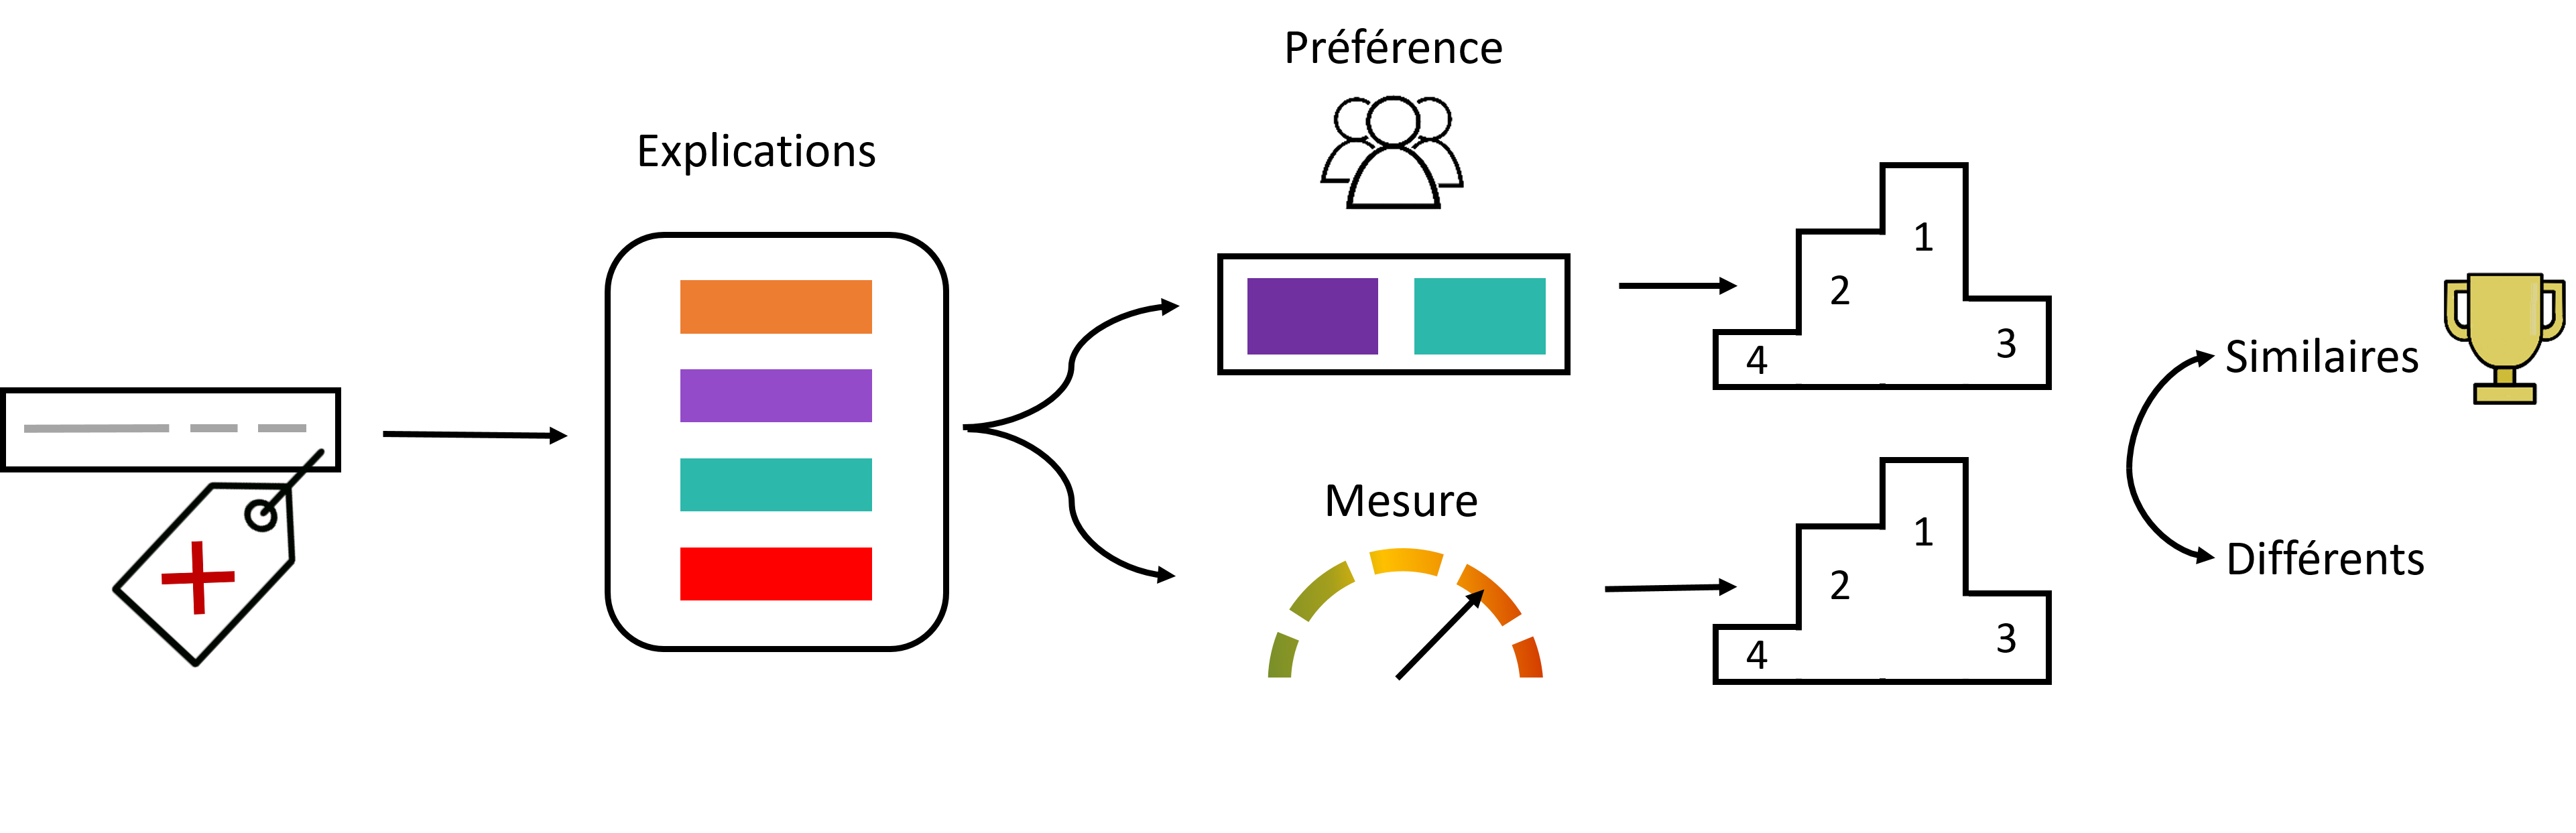
\includegraphics[width=\textwidth]{S3-Comparaison_de_methodes/figures/experiment.png} %
  \caption{Processus global de l'expérience, avec étude psychométrique des utilisateurs et analyse quantitative.}\label{fig:experiment}
 \end{center}
\end{figure}

Tout d'abord, des données étiquetées sont fournies au modèle et aux méthodes d'explication à évaluer. Comme la comparaison par paires est réalisée plus tard, nous recommandons de ne considérer que quelques méthodes d'explication évaluées à la fois.

Pour obtenir la métrique quantitative, les explications générées sont comparées à la référence.
La première version est une métrique simple, ici l'IOU comme vu dans la section~\ref{C3:qt_metric}. Encore une fois, la référence est considérée comme la meilleure option par conception et obtient le score maximal de 1. Les autres explications obtiennent des scores compris entre 0 et 1, 1 étant le meilleur. En classant les méthodes d'explication par leur score moyen, on obtient le classement quantitatif.

La comparaison par paires du chapitre précédent donne une matrice de préférences. L'élément $i,j$ de cette matrice indique le nombre de fois où $i$ a été préféré à $j$. Pour obtenir un classement à partir de cette matrice, l'algorithme Bradley-Terry-Luce (BTL)~\cite{Bradley1952,Luce1959} est utilisé. Il permet de transformer une matrice de comparaison par paires en un classement ordonné de tous les éléments comparés. Nous obtenons ainsi une échelle psychométrique ordonnant les quatre méthodes d'explication : la référence et les explications générées.

Une fois les podiums définis, nous pouvons les comparer. Si le classement de la métrique quantitative est similaire aux préférences humaines, nous pouvons estimer sans risque que la métrique reflète les préférences des utilisateurs. La métrique peut être conservée et réutilisée avec d'autres méthodes d'explication si nécessaire.
Si le classement de la métrique quantitative n'est pas similaire aux préférences des utilisateurs, alors notre métrique quantitative doit être améliorée. Une analyse des données de cette expérience donnera des pistes sur ce qu'il faut améliorer.

Ce protocole est appliqué au cas d'usage LEGO. Toutefois, il doit être adapté pour chaque cas d'usage, avec si besoin un format de données différent, un nombre variable de méthodes d'explication, et une métrique quantitative personnalisée.

% Les données consistent ici en des phrases d'offres d'emploi comme entrées textuelles avec leurs étiquettes associées : raison du rejet.

La génération des explications est décrite dans le chapitre précédent. Comme les ancres doivent être générées avec un modèle, le modèle d'attention est utilisé pour générer l'étiquette. Cela garantit que les différences de modèle n'auront pas d'impact sur l'expérience. Dans ce travail, nous comparons les ancres et deux explications de l'attention avec des seuils de valeurs $t = 0,15$ et $t = 0,5$. La deuxième explication avec un seuil $t = 0,5$ est générée spécifiquement pour cette expérimentation. Comme seul le seuil est plus élevé, les explications avec \textit{attention 0,5} sont un sous-ensemble des explications avec \textit{attention 0,15}, avec les mêmes mots ou plus concises. Elles permettent d'étudier le niveau d'information attendu par les utilisateurs. Pour chaque phrase, une explication de référence par attention humaine est également établie, tous les détails sont donnés dans la section~\ref{C2:ground_truth} du chapitre précédent. Une entrée génère quatre éléments à comparer.
% conclusion et prochaine section
Maintenant que l'expérience globale a été présentée, nous procédons à la mesure quantitative de qualité des explications.

\subsection{Mesure quantitative}\label{C3:iou_lego_de}

% Pourquoi
Dans l'expérimentation précédente (cf. section~\ref{C3:iou_expe}) sur le jeu de données LEGO - BP, nous avons considéré la performance des explications en tant que similarité entre explication générées et de référence. Cette similarité est mesurée avec l'IOU. Dans la section courante, nous effectuons cette même mesure, cette fois sur le jeu de données LEGO - DE, puisque la collecte des préférences utilisateurs contraint à ne pas avoir 2 fois la même explication,

La comparaison de la métrique quantitative avec les préférences utilisateurs implique de recalculer l'IOU dans ce jeu de données pour définir le podium de la métrique quantitative.
En raison de cette variation dans la conception du jeu de données, une baisse conséquente de l'IOU est attendue par rapport à l'IOU calculé sur le jeu de données LEGO BP dans la section~\ref{C3:iou_expe} : les phrases conformes du jeu de données LEGO - BP ne sont plus présentes dans le jeu de données LEGO - DE, et tiraient les résultats vers le haut. Le jeu de données LEGO - DE ne contient lui aucune phrase conforme.

% Comment
L'IOU est calculé avec le même protocole qu'en section~\ref{C3:iou_expe}, les mots d'arrêt étant ignorés. Comme le montre la première ligne du tableau~\ref{iou_lego_de_cplx}, les scores baissent de manière significative par rapport aux chiffres présentés dans le tableau~\ref{anchors_gt_lego_success} ce qui était attendu.

Une analyse plus poussée montre que, dans notre cas, cette baisse est principalement due au fait de prendre en compte les cas où le modèle de prédiction est en échec, ces cas étant filtrés dans le jeu de données LEGO - BP. Ainsi, l'IOU entre les ancres et les explications de référence pour le jeu de données DE est en moyenne de $0,27$. Pour les cas où le modèle est en succès elle est en moyenne de $0,52$, pour les cas où il est en échec, l'IOU est de $0,02$.

% Résultats et analyse
\begin{table}[h!tpb]
  \centering
  \addtolength{\parskip}{-0.5mm}
\caption{Comparaison objective des ancres et des explications d'attention. Les explications sont comparées à la référence avec l'IOU, sur le jeu de données LEGO - DE.}\label{iou_lego_de_cplx}
\begin{tabular}{|l|l|c|c|c|}
  \hline
  \textbf{Type d'explication} & \textbf{Ancres} & \textbf{Attention 0,15} & \textbf{Attention 0,5} \\ \hline
  Total  (106)  & 0,27 & 0,23 & 0,23 \\ \hline \hline
  Vide (53) & 0,02 & 0,13 & 0,21 \\ \hline
  Simple (12) & 0,53 & 0,58 & 0,46 \\ \hline
  Complexe (41) & 0,51 & 0,25 & 0,20 \\ \hline
\end{tabular}
\end{table}

La première ligne du tableau~\ref{iou_lego_de_cplx} montre une faible différence entre les méthodes. Une analyse plus poussée dans ce cas d'usage implique de différencier les phrases en fonction de leur explication de référence, cette analyse est présentée dans les lignes suivantes du tableau~\ref{iou_lego_de_cplx}. Les phrases conformes n'ont pas de référence. Ces phrases constituent la catégorie d'explication \textit{vide}. Certaines phrases ont des explications attendues \textit{simples}, composées d'un ou deux mots. Enfin, nous regrouperons les explications attendues de trois mots ou plus dans la catégorie \textit{complexe}. Ce regroupement nous donne les scores moyens de similarité pour la Figure~\ref{fig:iou_plot_cplx}.

\begin{figure}[h!tpb]
  \setlength{\belowcaptionskip}{-20pt}
 \begin{center}
  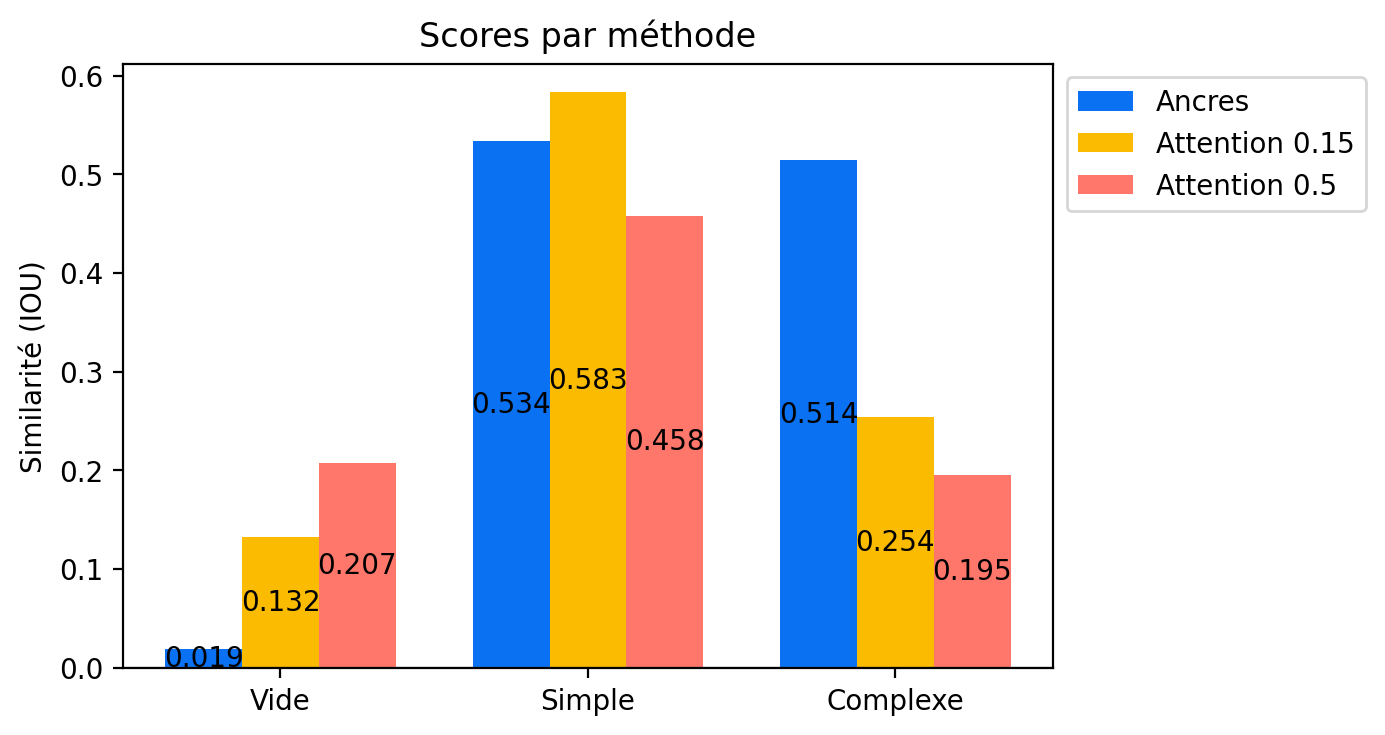
\includegraphics[width=0.9\textwidth]{S3-Comparaison_de_methodes/figures/iou_by_complexity.png}
  \caption{Scores moyens de similarité aux explications de référence, obtenus avec l'IOU pour chaque méthode d'explication, sur le jeu de données LEGO DE.} \label{fig:iou_plot_cplx}
 \end{center}
\end{figure}

Le premier groupe de la figure~\ref{fig:iou_plot_cplx} montre que les trois explications générées ont une faible IOU, en particulier la méthode des ancres. Cela s'explique par le fait que l'IOU avec une explication de référence vide ne peut être que de 0 ou 1. Une IOU de 0 est obtenue lorsqu'une méthode donne n'importe quel mot comme explication, donc l'intersection de cette explication et de l'absence d'explication est de longueur 0. Lorsqu'une méthode ne donne aucune explication, nous comparons deux ensembles vides. Comme ils sont égaux, l'IOU est égale à 1. Comme les méthodes des ancres et d'attention ne donnent rarement aucune explication, leur IOU est très faible par rapport à l'explication humaine, vide.
Le deuxième groupe met en évidence les bonnes performances des méthodes des ancres et d'attention avec $t=0.15$ pour imiter l'explication humaine donnée. Le dernier groupe, pour les cas complexes, indique une divergence significative des deux méthodes d'attention par rapport à l'explication humaine. Cependant, la méthode des ancres conserve une IOU stable entre le 2ème et le 3ème groupe.

\begin{table}[h!tpb]
    \centering
    \addtolength{\parskip}{-0.5mm}
  \caption{Podium basé sur la mesure de similarité, sur le jeu de données LEGO DE, par catégorie d'explication. l'explication humaine sert de référence pour le calcul de l’IOU, elle n'apparaît donc pas dans ce tableau.}\label{qtm_podium}
\begin{tabular}{|l|l|l|l|}
    \hline
        & \textbf{Premier}  & \textbf{Second} & \textbf{Troisième} \\ \hline
Vide     &  Attention 0.5  & Attention 0.15  & Ancre         \\ \hline
Simple   &  Attention 0.15 & Ancre          & Attention 0.5  \\ \hline
Complexe &  Ancre         & Attention 0.15  & Attention 0.5  \\ \hline
\end{tabular}
\end{table}

% conclusion et transition
En définitive, les scores obtenus peuvent être traduits dans le podium du Tableau~\ref{qtm_podium}. Pour rappel, les explications de référence servent au calcul de l'IOU, elles sont considérées comme les meilleures explications pour chaque cas.
Nous avons donc un classement avec l'explication humaine, et les trois autres méthodes dans l'ordre comme indiqué dans le tableau~\ref{qtm_podium}. Ces podiums peuvent maintenant être comparés aux podiums des préférences des utilisateurs. Ces préférences utilisateurs sont abordées dans la section suivante.

\subsection{Préférences des experts} \label{C3:pref_humaine}

% Quoi
Dans cette section, nous classons les types d'explications étudiés selon les préférences des experts du domaine. Nous nous appuyons sur les comparaisons par paires dont la collecte est détaillée dans le chapitre précédent en section~\ref{C2:collect_pref}.
Ces comparaisons permettent le calcul du classement global des méthodes.

% Pourquoi
Ce classement des préférences des experts sera par la suite comparé aux mesures quantitatives. Toutefois en l'état, les comparaisons par paires ne donnent pas de comparaison globale des méthodes d'explications. Nous allons donc dans cette section transformer ces comparaisons par paires en classement global.

% Comment
$A = (a_{ij})_{m \times m}$ est la matrice de préférences issue de la collecte de comparaisons par paires. Chaque coefficient $a_{ij}$ est le nombre de fois où le stimulus (l'explication) $S_i$ a été préféré au stimulus $S_j$. La diagonale de la matrice est nulle.
Le nombre de comparaisons est $n_{ij} = a_{ij}+a_{ji}$ et la probabilité que $S_i$ soit préféré à $S_j$ est $P_{ij} = a_{ij}/n_{ij}$.

Nous obtenons un score de crédit $v_i$ à partir de la matrice de préférences grâce au modèle BTL~\cite{Bradley1952,Luce1959}. Ce modèle se base sur les comparaisons par paires pour estimer les scores $v_i$ selon l'équation~\ref{eq:btl}. Ils sont calculés itérativement pour tous les éléments $i$, puis normalisés en les divisant par la somme des $v_i$, jusqu'à ce que les scores convergent à un état stable.
\begin{equation} \label{eq:btl}
    v_i = \frac{A_i}{\sum_{j \neq i \frac{a_{ij}+a_{ji}}{v_i + v_j}}}
\end{equation}

Ici, le score de crédit $v_i$ représente la probabilité qu'un utilisateur choisisse une méthode plutôt que les autres. Pour un stimulus donné $i$, $A_i$ est la somme des $a_{ij}$ pour tout $j$.
On obtient alors une échelle psychométrique telle que celle de la figure~\ref{fig:btl_plot}. Un score plus élevé indique la préférence des utilisateurs. Comme le score $v_i$ est calculé par rapport aux autres éléments, il n'est pas possible de comparer les scores des éléments $i$ d'une comparaison, avec les éventuels scores $v_k$ obtenus par l'application du BTL à un ensemble différent d'éléments.

% Résultats et analyse
Nous illustrons le calcul des scores avec le cas d'usage LEGO. Les scores BTL peuvent être évalués par phrase. Comme le montre la figure~\ref{fig:btl_plot}, pour cette phrase spécifique, l'échelle psychométrique indique l'ancre comme méthode préférée, et l'explication humaine comme moins appréciée par les utilisateurs.

\begin{figure}[h!tpb]
  \setlength{\belowcaptionskip}{-20pt}
\begin{center}
  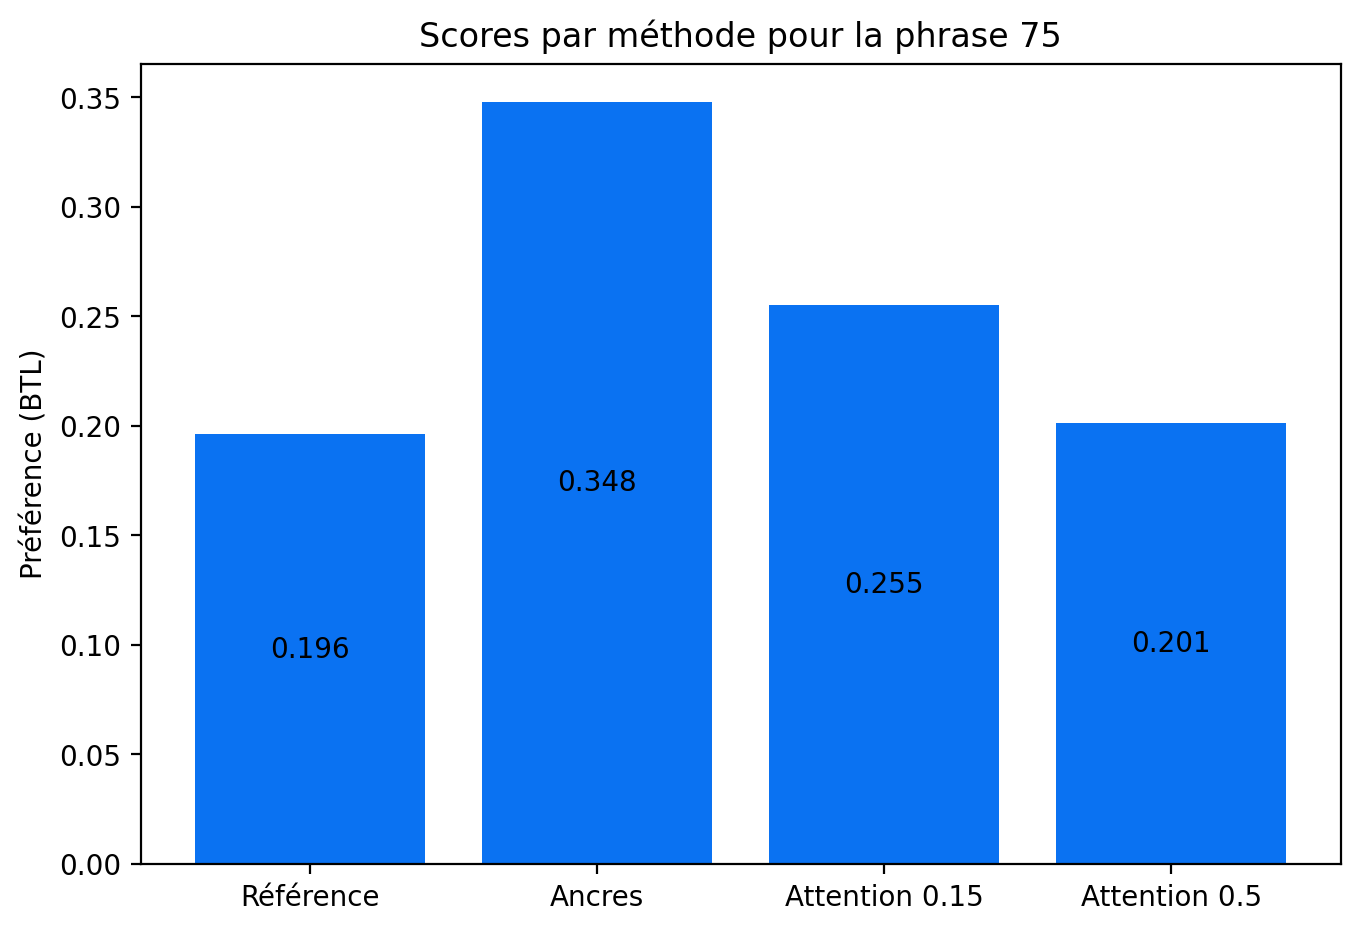
\includegraphics[width=0.68\textwidth]{S3-Comparaison_de_methodes/figures/btl_plot.png}
  \caption{Exemple des scores obtenus avec le modèle BTL pour chaque méthode d'explication sur une phrase du jeu de données LEGO - DE. La valeur correspond à la probabilité qu'un utilisateur préfère une méthode plutôt que les autres. L'explication humaine correspond à la colonne ``Référence''. }\label{fig:btl_plot}
 \end{center}
\end{figure}

Nous observons ensuite les scores BTL sur l'ensemble du jeu de données LEGO DE, et sur deux sous-ensembles : les vrais positifs et les faux positifs, car nous nous attendons à ce que les résultats diffèrent. Les résultats sont comparés dans la figure~\ref{fig:btl_plot_global}. Cette analyse ne montre aucune différence significative entre les méthodes, autant sur la base complète que sur les deux sous-ensembles. Un tel résultat souligne que, sur le plan global, aucune méthode ne l'emporte en termes de préférence utilisateur.

\begin{figure}[h!tpb]
  \setlength{\belowcaptionskip}{-20pt}
 \begin{center}
  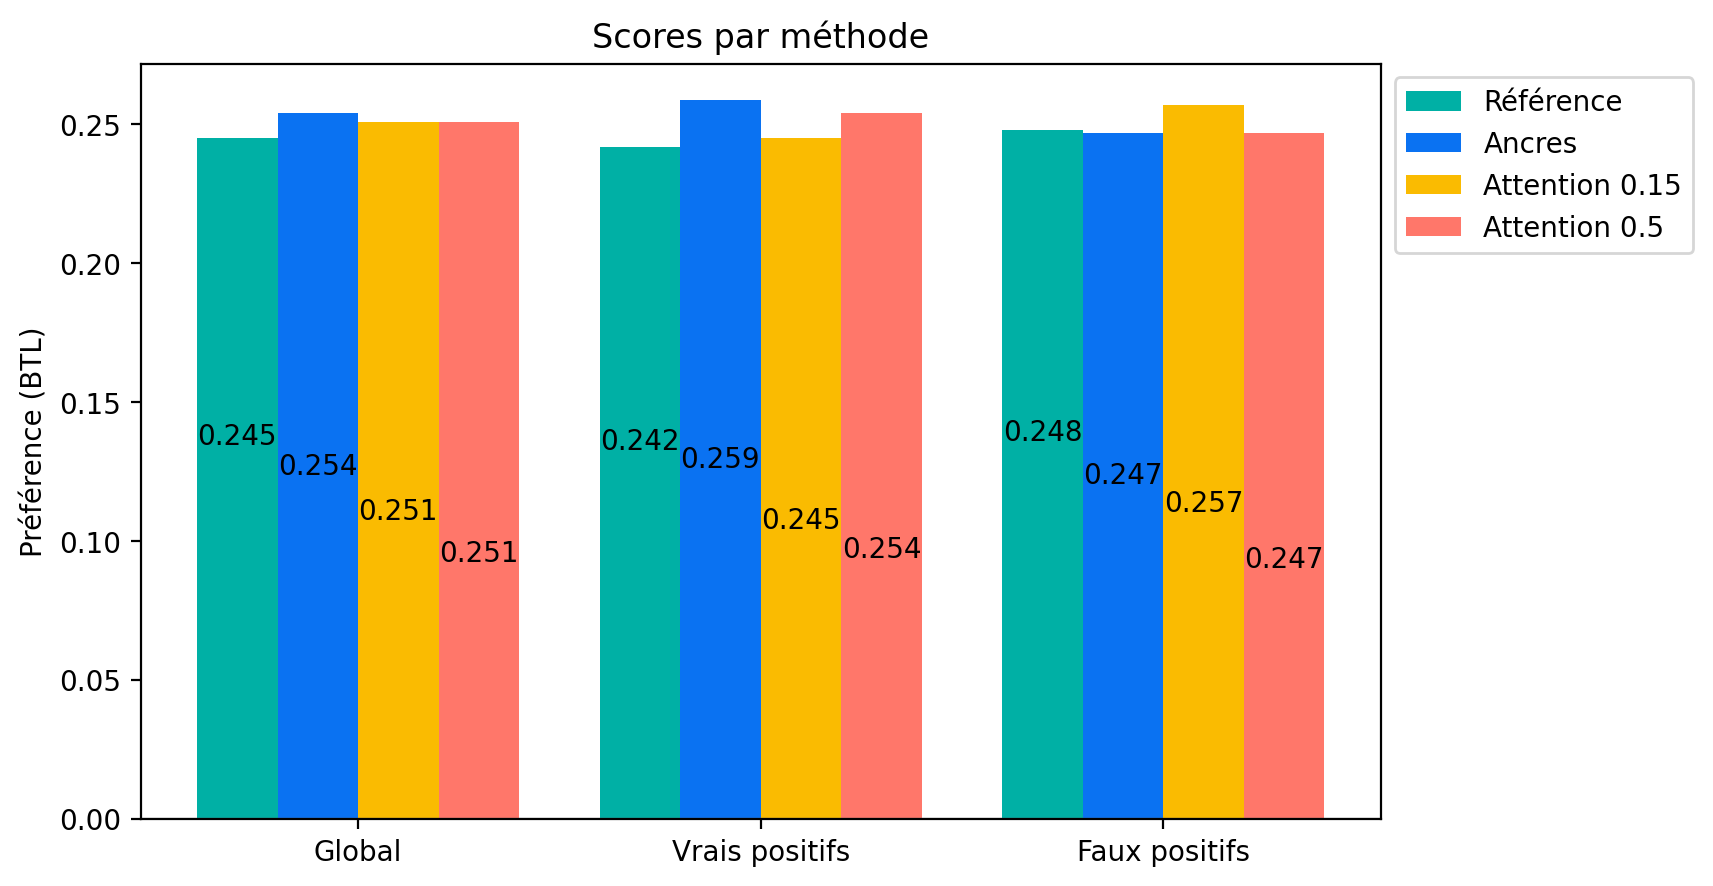
\includegraphics[width=0.9\textwidth]{S3-Comparaison_de_methodes/figures/btl_plot_global_tp_fp.png}
  \caption{Scores obtenus avec le modèle BTL pour chaque méthode d'explication, sur le jeu de données LEGO DE. Les vrais positifs et les faux positifs sont indiqués. Aucune différence significative n'apparaît entre les méthodes.}\label{fig:btl_plot_global}.
 \end{center}
\end{figure}

Comme nous l'avons fait dans la section~\ref{C3:iou_lego_de}, nous allons diviser notre ensemble de données par phrases avec des explications de référence \textit{vide}, \textit{simple} et \textit{complexe}. L'algorithme BTL nous donne l'échelle psychométrique associée dans la Figure~\ref{fig:btl_plot_cplx}.

\begin{figure}[h!tpb]
  \setlength{\belowcaptionskip}{-20pt}
 \begin{center}
  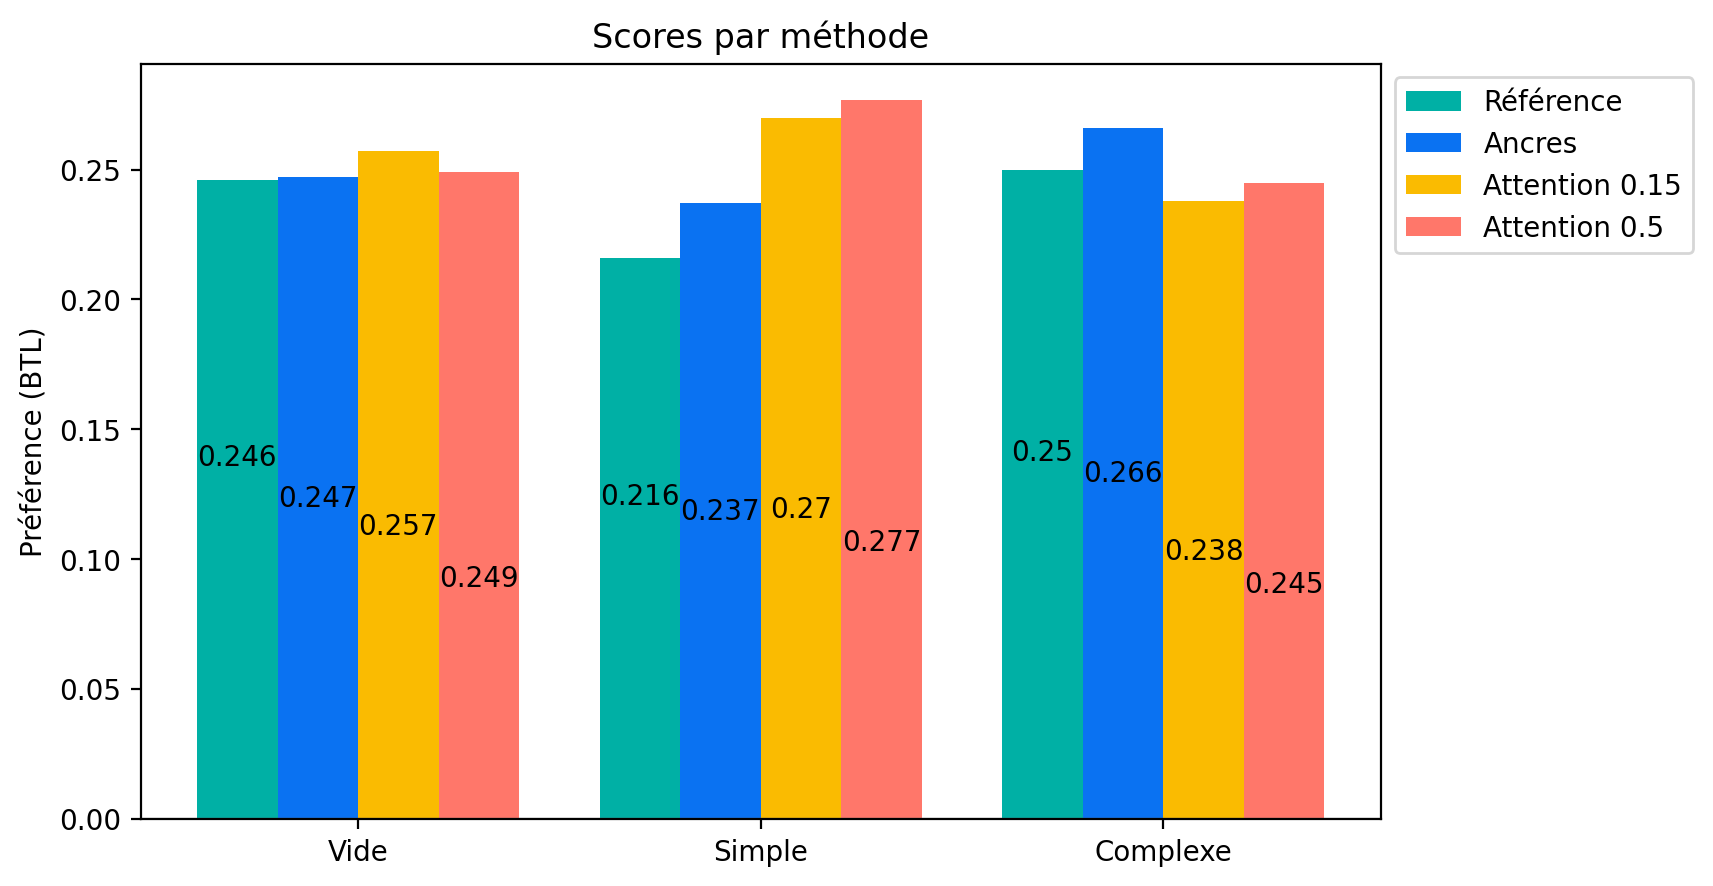
\includegraphics[width=0.9\textwidth]{S3-Comparaison_de_methodes/figures/btl_by_complexity.png}
  \caption{Scores obtenus avec le modèle BTL pour chaque méthode d'explication, sur le jeu de données LEGO DE, par complexité. Ce regroupement montre des différences dans les préférences des utilisateurs. }\label{fig:btl_plot_cplx}
 \end{center}
\end{figure}

Encore une fois, cette échelle psychométrique peut être transformée en podiums, affichés dans le tableau~\ref{pus_podium}. Faisons la première analyse pour tous les types de phrases. Pour les phrases avec une explication de référence vide, les utilisateurs n'ont pas une forte préférence pour une méthode ou une autre, comme le montre la Figure~\ref{fig:btl_plot_cplx}. Le podium dans le tableau~\ref{pus_podium} indique que la légère préférence va aux méthodes d'attention.
Pour les cas simples, les méthodes d'attention interne sont préférées, et l'explication humaine est la moins appréciée. Pour les cas plus complexes, la méthode d'explication des ancres a été préférée, et les méthodes d'attention interne sont en difficulté. Dans notre cas d'usage, en d'autres termes, les utilisateurs préfèrent les méthodes d'attention dans les cas simples. Lorsque les choses deviennent plus complexes, leur préférence va à la méthode d'explication des ancres.

\begin{table}[h!tpb]
    \centering
    \addtolength{\parskip}{-0.5mm}
  \caption{Podium basé sur une étude psychométrique des utilisateurs, sur le jeu de données LEGO DE, par catégorie d'explication.} \label{pus_podium}
  \begin{tabular}{|l|l|p{0.25\textwidth}|l|l|}
      \hline
           & \textbf{Premier}& \textbf{Second}   & \textbf{Troisième} \\ \hline
  Vide     &  Attention 0,15 &  (Attention 0,5 ,  Ancre , Référence)  &&   \\ \hline
  Simple   &  Attention 0,5  &  Attention 0,15     & Ancre      &   Référence    \\ \hline
  Complexe &  Ancre          & Référence      &  Attention 0,5      &   Attention 0,15      \\ \hline
  \end{tabular}
  \end{table}

% Conclusion et transition
Nous avons calculé les préférences de chaque méthode d'explication et établi des podiums. L'analyse des résultats montre que différentes catégories de phrases existent et amènent des différences dans les préférences utilisateurs. Les podiums ainsi obtenus par catégorie sont comparés aux podiums de la métrique qualitative dans la section suivante.

\subsection{Résultats} \label{C3:pus_result}

% Quoi
Nous pouvons maintenant comparer les résultats de l'analyse quantitative de la section~\ref{C3:qt_metric} et les préférences des utilisateurs.
% Comment
Comme nous l'avons fait précédemment, nous regroupons les phrases par la complexité des explications de référence selon trois groupes : explications \textit{vides}, \textit{simples}, et \textit{complexes}.
Nous souhaitons désormais savoir si les méthodes d'explication qui performent le mieux sont également celles préférées par les humains.

% résultats
Les podiums du Tableau~\ref{qtm_podium} et du Tableau~\ref{pus_podium} présentés dans les sections précédentes diffèrent fortement. En effet, la métrique de similarité est basée sur les explications humaines en tant que référence, qui n'est pas la méthode préférée des utilisateurs.
Le diagramme à barres empilées tel qu'indiqué dans la Figure~\ref{fig:iou_btl_e} permet de comparer la proportion relative des méthodes dans chaque cas. Les valeurs de similarité par IOU sont normalisées pour la comparaison, afin que la somme de tous les scores soit égale à un. Les valeurs réelles sont présentées dans le tableau~\ref{iou_lego_de_cplx}.

Pour les phrases de catégorie \textit{vides}, la figure~\ref{fig:iou_btl_e} montre que l'IOU et BTL reflètent des explications différentes. Pour rappel, le jeu de données DE est composé de phrases étiquetées comme non conformes par notre modèle. Les explications de référence vides sont associées à des phrases conformes, qui ont été prédites à tort comme non conformes par le modèle. Dans ce cas, les explications humaines telles que nous les avons définies peuvent ne pas être la bonne référence pour calculer les IOU. Comme expliqué dans la section~\ref{C2:ground_truth}, les experts du domaine pourraient préférer une explication attendue, qui devrait être définie pour un modèle spécifique.

\begin{figure}[h!tpb]
  \setlength{\belowcaptionskip}{-0pt}
 \begin{center}
  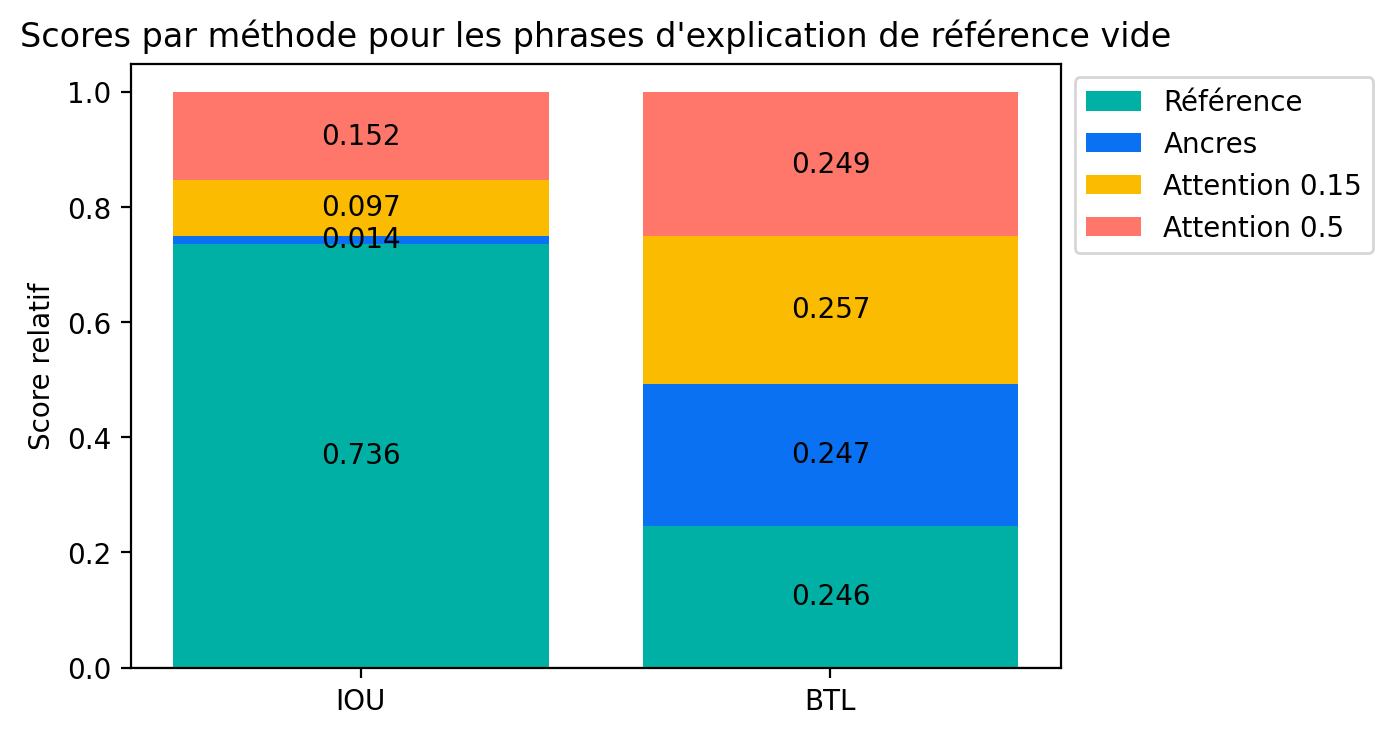
\includegraphics[width=0.8\textwidth]{S3-Comparaison_de_methodes/figures/iou_btl_e.png}
  \caption{Scores relatifs de similarité (IOU) et de préférence (BTL) normalisés pour chaque méthode d'explication, sur le jeu de données LEGO DE, filtré sur les phrases avec des explications vides. }\label{fig:iou_btl_e}
 \end{center}
\end{figure}

Le cas des phrases associées à des explications humaines \textit{simples} est présenté dans la figure~\ref{fig:iou_btl_s}. Elle met en évidence de bons résultats quantitatifs pour l'\textit{attention 0,15} et les ancres, l'\textit{attention 0,5} étant la méthode qui correspond le moins à l'explication humaine. Les utilisateurs n'ont pas préféré l'explication humaine aux autres méthodes et ont préféré l'\textit{attention 0,5}. Prendre l'explication humaine comme référence n'a donc pas de sens, et nous pouvons en conclure que l'IOU basée sur l'explication humaine n'est pas efficace ici non plus. Cependant, les utilisateurs semblent apprécier les explications courtes, puisqu'iels ont préféré \textit{attention 0,5} à \textit{attention 0,15}. Notre métrique quantitative devrait refléter ce point, en diminuant lorsque la longueur d'une explication augmente.

\begin{figure}[h!tpb]
  \setlength{\belowcaptionskip}{-20pt}
 \begin{center}
  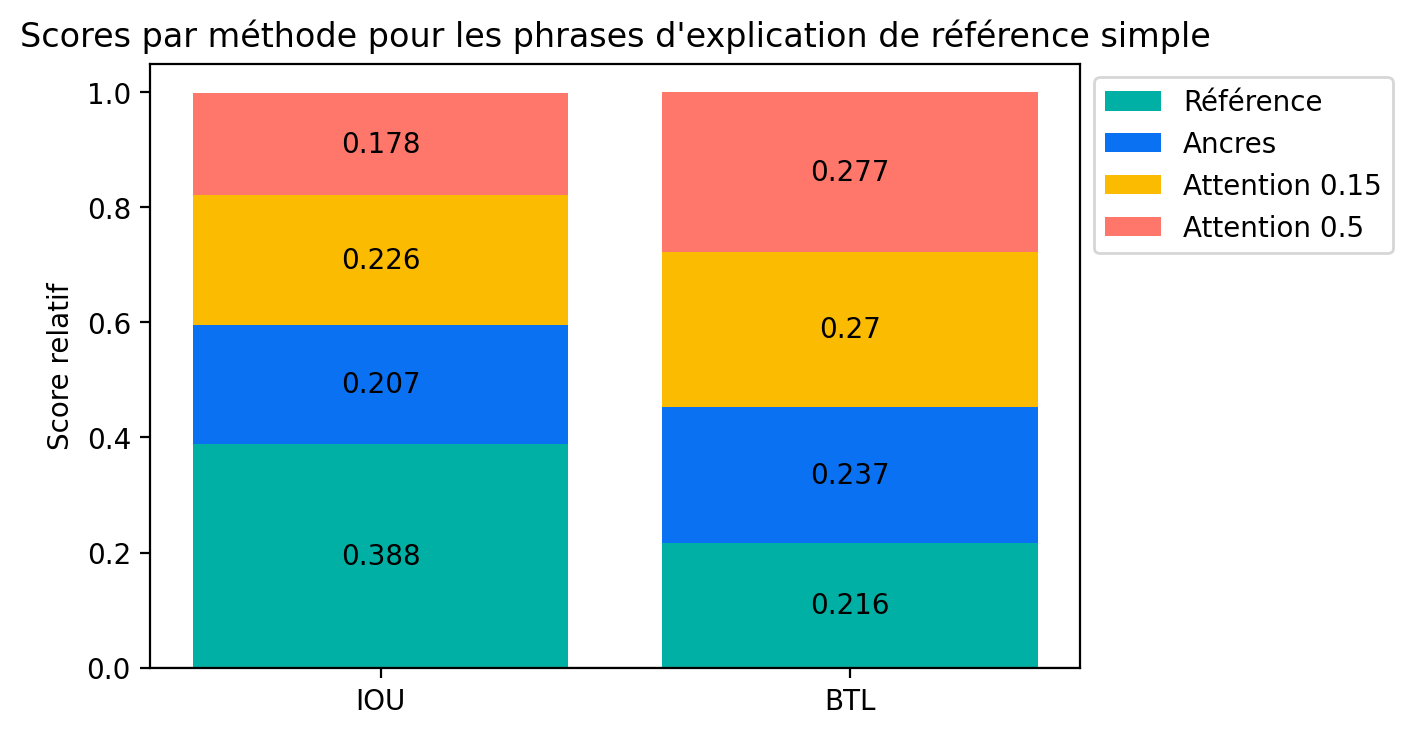
\includegraphics[width=0.8\textwidth]{S3-Comparaison_de_methodes/figures/iou_btl_s.png}
  \caption{Scores relatifs de similarité (IOU) et de préférence (BTL) normalisés pour chaque méthode d'explication, sur le jeu de données LEGO - DE, filtré sur les phrases avec des explications simples. Les explications de référence sont d'IOU égale à $1$ avant normalisation.  }\label{fig:iou_btl_s}
 \end{center}
\end{figure}

Les podiums pour les phrases avec des explications de référence plus complexes sont comparés dans la figure~\ref{fig:iou_btl_c}. L’IOU montre une bonne correspondance pour les explications des ancres. Cela se reflète dans l'étude des utilisateurs, puisque la méthode préférée est celle des ancres, suivie de la référence. En considérant l’IOU, l'\textit{attention 0.5} est moins performante comparée à \textit{attention 0.15}. Cependant la préférence des utilisateurs est inverse. Comme l'\textit{attention 0,5} est un sous-ensemble de \textit{attention 0,15}, cela indique une préférence pour les explications plus courtes. Tout comme pour les cas simples, notre métrique refléterait mieux les préférences des utilisateurs en tenant compte de la longueur des explications.

\begin{figure}[h!tpb]
  % \setlength{\belowcaptionskip}{-20pt}
 \begin{center}
  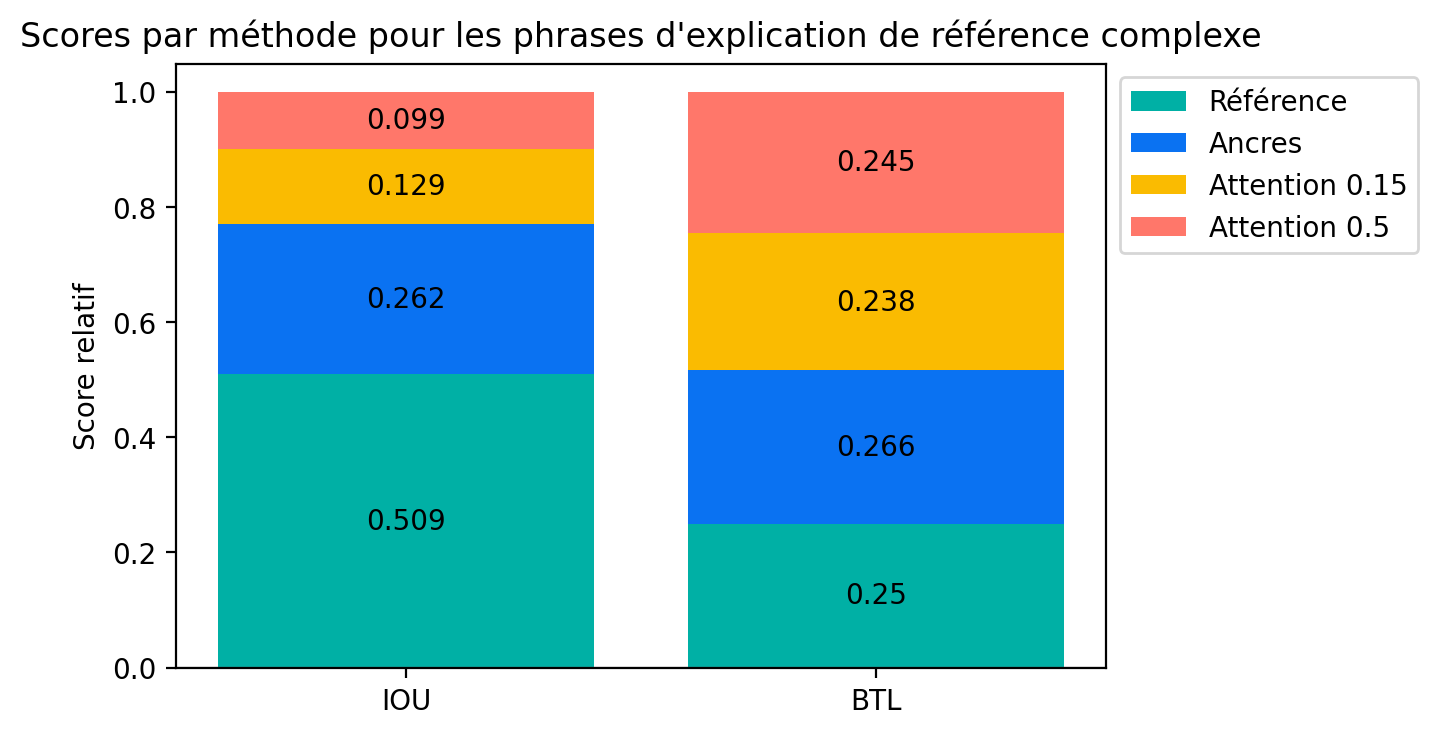
\includegraphics[width=0.8\textwidth]{S3-Comparaison_de_methodes/figures/iou_btl_c.png}
  \caption{Scores relatifs de similarité (IOU) et de préférence (BTL) normalisés par méthode d'explication, sur le jeu de données LEGO DE, filtré sur les phrases avec des explications complexes. }\label{fig:iou_btl_c}
 \end{center}
\end{figure}

Pour toutes ces catégories, nos podiums sont différents. Selon notre protocole, cela signifie que notre mesure quantitative ne reflète pas la préférence humaine. Pour ajuster cette mesure, l'analyse des résultats donne deux pistes.
\begin{itemize}
    \item Les explications attendues sont plus pertinentes que les explications idéales (Cf. section~\ref{C2:ground_truth}) pour mesurer la préférence des utilisateurs.
    \item Prendre en compte la préférence des utilisateurs pour les explications courtes.
\end{itemize}
Nous répondons à notre seconde question : ``comment faire pour que la métrique quantitative corresponde aux préférences des utilisateurs?'' par une nouvelle mesure de performance.
% \begin{equation}\label{qtm_iou}
%   metrique = \frac{e_{generee} \cap e}{e_{ideale} \cup e}
% \end{equation}
% à
\begin{equation}\label{qtm_new}
  performance = \frac{e_{generee} \cap e}{e_{attendue} \cup e} \frac{\alpha}{len(e)}
\end{equation}

\section{Conclusion}

% Objectif  du chapitre
Nous avons collecté en section~\ref{C3:test_u} les retours des utilisateurs dans la conception des systèmes d'explications. Nous avons ensuite présenté les comparaisons de méthodes de génération d'explications, dans deux contextes : sans utilisateurs en section~\ref{C3:iou_expe} et avec en section~\ref{C3:pus}. Les protocoles ont été conçus pour être généralisés à tout cas d'usage de classification multi-classe. Ils sont applicables à toute méthode d'explication par variable d'importance.

% on en retire quoi, limites
Le test d'utilisabilité a donné l'idée d'une interface non envisagée avant : l'explication par la règle. Il a démontré son intérêt tout en nécessitant peu de temps de réalisation.

La comparaison sans utilisateurs donne des résultats différents selon le cas d'usage.
Pour le second protocole, les résultats montrent que la méthode préférée dépend de la taille de l'explication de référence. Les explications de référence ne sont pas représentatives des préférences des utilisateurs. Les utilisateurs préfèrent des explications courtes.

Cette mise en pratique met en lumière la dépendance de ces méthodes d'évaluation à la disponibilité et la qualité d'explications de référence. Sans ces explications les évaluations sont restreintes et nécessitent une analyse manuelle qui, bien que rendue la plus efficiente possible, reste lourde.
Les faux positifs sont une source de différence entre les explications attendues et les explications idéales, et cibler ceux-ci peut réduire le coût de passer d'explications idéales à attendues.

% et on discute de la suite
Nous avons évalué le format et les méthodes de génération d'explications locales. Dans le chapitre suivant, nous nous attelons à générer des explications globales sur le comportement d'un modèle.

\boitemagique{Résumé}{
\begin{itemize}
    \item[\checkmark] Nous avons collecté les besoins des experts du domaine
    \item[\checkmark] Les systèmes d'explications les plus complexes ne mènent pas aux interfaces les plus appréciées des utilisateurs
    \item[\checkmark] L'évaluation des explications sans avis humain permet une première mesure de d'adéquation
    \item[\checkmark] L'évaluation subjective permet de tenir compte les préférences des experts dans la mesure de performance
    \item[\checkmark] Le protocole d'évaluation a mené aux publications~\cite{Jouis2021,Jouis2021a,Jouis2023}
\end{itemize}
}
